\documentclass[letterpaper]{article}
\usepackage{natbib,alifeconf}
\usepackage{hyperref}

\title{What is necessary for open-ended evolution?}
\author{Anya E. Vostinar$^{1,2,3,*}$, Emily L. Dolson$^{1,2,3,*}$, Michael J. Wiser$^{1,3}$,\and Charles Ofria$^{1,2,3}$ \\
\mbox{}\\
$^1$BEACON Center for the Study of Evolution in Action  \\
$^2$Department of Computer Science and Engineering, Michigan State University \\
$^3$Program in Ecology, Evolutionary Biology, and Behavior, Michigan State University \\
ofria@msu.edu\\
$^*$Authors contributed equally}



\begin{document}
\maketitle


\section{Introduction}

    A central goal of the field of artificial life is to build evolving systems that capture interesting dynamics of natural systems, producing evolutionary outcomes such as sophisticated navigation behaviors, novel cooperative strategies, complex ecosystems, or major evolutionary transitions, to name but a few. Such ``open-ended'' systems are sought after for a number of reasons: 1) For artificial life researchers, the presence of dynamics that are seen in biology but not artificial life raises the possibility that there is some fundamental and as-of-yet unidentified quality that artificial life systems are missing (citation). 2) For biologists, access to systems exhibiting complex and nuanced evolutionary processes allows rapid experimentation and facilitates understanding them on a mechanistic level (citations). 3) For evolutionary computation researchers, insights from open-ended evolutionary systems have the potential to expand the classes of applied engineering problems that we are able to solve with evolutionary algorithms (citations). Biological evolution is the only process known to have produced general intelligence; replicating this process would provide incredible insights into our own origins, as well as allowing us to harness these dynamics to spur breakthroughs in artificial intelligence. While various artificial life systems have recreated individual dynamics -- such as the evolution of complexity, cooperation, and competition (citations) -- these accomplishments have been in highly controlled circumstances. The overarching goal of open-ended evolution research is to create a system where all of these dynamics can emerge more organically, as in the biosphere. 
    
Despite general agreement on open-ended evolution being an important goal in artificial life, the field has yet to come to a consensus on how to define whether systems are making progress towards achieving this goal. A number of dynamics have been proposed as being possibly necessary for open-ended evolution, most notably the continuous production of novelty (cite Stanley and maybe Banzhaf if he’s published that paper yet), the continuous increase in diversity (cite Bedau and maybe others), the continuous increase in complexity (citations), and shifts in individuality such as those often associated with major transitions in evolution (cite maynard smith, ackley if he has a paper). We argue that all of these dynamics are important pieces of the open-ended evolution puzzle. In addition, we have previously suggested that there is a fifth necessary and even simpler dynamic: continuous change in the population (cite blog post).

\begin{figure}
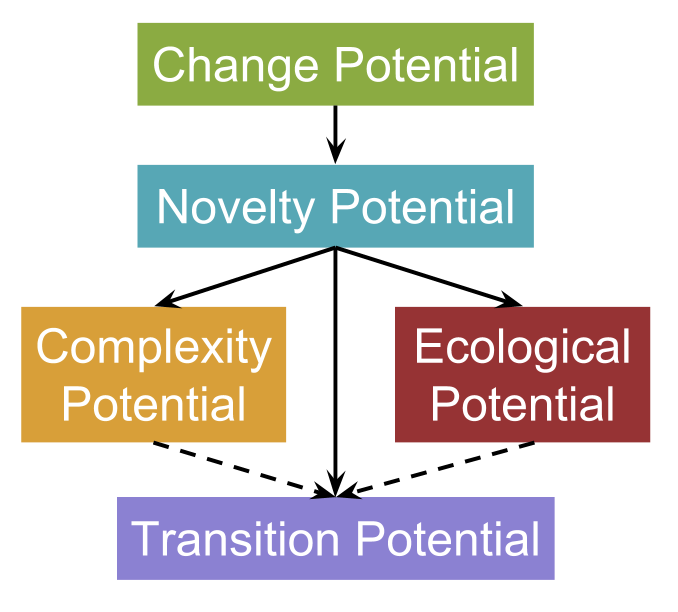
\includegraphics[width=3.5in]{figs/Complexity_Barriers.png}
\caption{\textbf{Relationships between the metrics.} }
\label{hierarchy}
\end{figure}
These five properties of a system fit into a hierarchy, as shown in Figure \ref{hierarchy}. For novelty to arise, there must be some degree of change in a population. While this is trivially true, many evolutionary algorithms suffer from premature convergence, which is essentially the absence of change, so it remains an important prerequisite to define and explicitly address. Similarly, complexity and diversity can only increase indefinitely if novel members of the population continue to be generated. Finally, transitions in individuality typically involve multiple organisms coming together into a single individual, requiring an increase in complexity and a diversity to build from.  All of these dynamics capture different subsets of interesting behavior that an evolving system might have and we propose they are all necessary for a system to demonstrate open-ended evolution.

To draw conclusions about what factors of a system promote or inhibit these dynamics, it is critical to first develop a common suite of metrics that are applicable across a wide variety of systems. Some progress has been made toward this end with evolutionary activity statistics (cite). Evolutionary activity statistics focus on ``components" representing the meaningful individual pieces of a system, which the authors admit will need to be defined for each system as appropriate. For instance, in the fossil record, species were used as components. Once these components are decided upon, the diversity and amount of adaptive evolutionary activity of components in a given time step are used to determine into which of three classes of evolution the system falls. These classes of evolutionary activity (none, bounded, unbounded) follow logically from whether diversity and novel evolutionary activity per component is bounded or unbounded. However, to filter out changes that do not represent adaptive evolutionary activity, a neutral ``shadow'' control with no selective pressure must be run for comparison. Creating a shadow control treatment can make implementing evolutionary statistics difficult in complex systems. Moreover, the need to select an appropriate component can make results challenging to generalize across systems. Lastly, evolutionary activity statistics may not be able to differentiate dynamics in which a subset of the population is gaining new and interesting traits from less interesting dynamics in which that subset is merely under stabilizing selection.

In this paper, we extend the ideas behind evolutionary activity dynamics. We propose to quantify the idea of open-ended evolution with a suite of four necessary but not always sufficient metrics that attempt to balance generalizability across systems with the ability to capture the ideas of the first four dynamics previously discussed: change, novelty, complexity, and ecological interactions. The novelty and ecological metrics track the same dynamics as new components and diversity in evolutionary activity statistics. Complexity provides a more direct measure of whether any part of the system is gaining interesting adaptations. We propose an alternative technique for isolating adaptive evolutionary activity, which we hope will be more widely applicable (see Persistent Lineages). Additionally, we propose a technique for selecting meaningful components that will work for any system in which genomes are composed of elements that collectively determine fitness (see Informative Sites). We present our results when applying these four metrics to an NK system.  The fifth metric, transition potential, has proven more difficult to quantify in such an intuitive and computationally tractable manner and we are reserving it for future study.


\section{Experimental System}
    To begin a systematic examination of our metrics, we used a simple NK model~\citep{kauffman_towards_1987}. An NK model uses two parameters, N and K, to randomly generate a fitness landscape. N specifies the number of sites in the genome, each of which is a 0 or a 1. The fitness landscape specifies the effect of a given value at a given site on the fitness of the bit-string organism. This fitness effect depends on the values at the K subsequent adjacent sites. As such, K tunes the ruggedness of the landscape; low values of K produce smooth landscapes with few peaks, whereas high values produce landscapes with many peaks. We chose to use an NK model because they are a well-understood system for studying general questions about evolutionary dynamics.

\subsection{Experimental Treatments}
	Our basic treatment used $N=20$ (i.e., 20 bits in an individual) and $K=3$ (the fitness contribution of each bit was influenced by three other bits).  We used a population size of 200 and a mutation rate of 3 sites (three bits were randomized in each birth, so a 1/8 chance of all three returning to their original values), with tournament selection and a tournament size of 15.  On top of this basic treatment, we performed eight experimental treatments: \textbf{High K} tests the effect of a highly rugged landscape (K=10) where fitness is effectively randomized whenever a mutation occurs.  \textbf{High N} tests the effect of longer bit-string genomes (N=100), allowing for a higher potential complexity.  \textbf{Low Mut} and \textbf{High Mut} test the effects of very low and very high mutations rates (1 bit and 6 bits, respectively), which we expect to be important for finding new areas of the fitness landscape and thus our noveltry metric.  \textbf{Small Pop} and \textbf{Large Pop} vary the population size (to 20 and 1000 respectively); in small populations we expect more drift in the population, allowing more change, while in a large population we expect stronger selection.  Finally, we did two special treatments: in \textbf{Changing Environmnents}, the fitness function was toggled every 500 generations, allowing us to see the effect of changing selective pressures where the popoulations couldn't stay on a single peak.  In \textbf{Fitness Sharing} organisms that were too similar to each other detracted from each others fitness, creating a pressure to explore multiple portions of the landscape at the same time and, ideally, maintain a high diversity.

\subsection{Persistent Lineages}
    At any given point in time, the population will contain some maladapted genomes that recently arose via mutation. These genotypes will quickly be purged from the population via natural selection and will add noise to our metrics. To decrease this noise, we must filter out such genomes. We accomplish this by looking backwards in time to see which organisms were the progenitors of lineages that persisted for a substantial number of generations. We mark each organism with a lineage number at a given time point A, as demonstrated in Figure~\ref{lineages} (where color indicates lineage number). The lineage numbers are passed on to offspring throughout the time interval (50 generations in our experiments). At time point A+50, we determine which genomes from the population at A have descendants at A+50. At this point, those genomes are considered \textbf{persistent}; in the example in Figure~\ref{lineages} the green and blue lineages are considered persistent at time point A+50. We then compare the green and blue genomes from time point A to the genomes that were persistent previously, either from time point A-50 or from all previous time points, depending on the metric; in the example we would compare to the purple genome at time point A-50. This filtering leads to a delay in counting a genome in a metric until 50 generations later, but enables us to avoid an apparent increase in metrics due to drift via mutation. For example, the red, orange, and blue genomes from time point A-50 would never be considered in our metrics because their lineages do not persist to time point A.

\begin{figure}
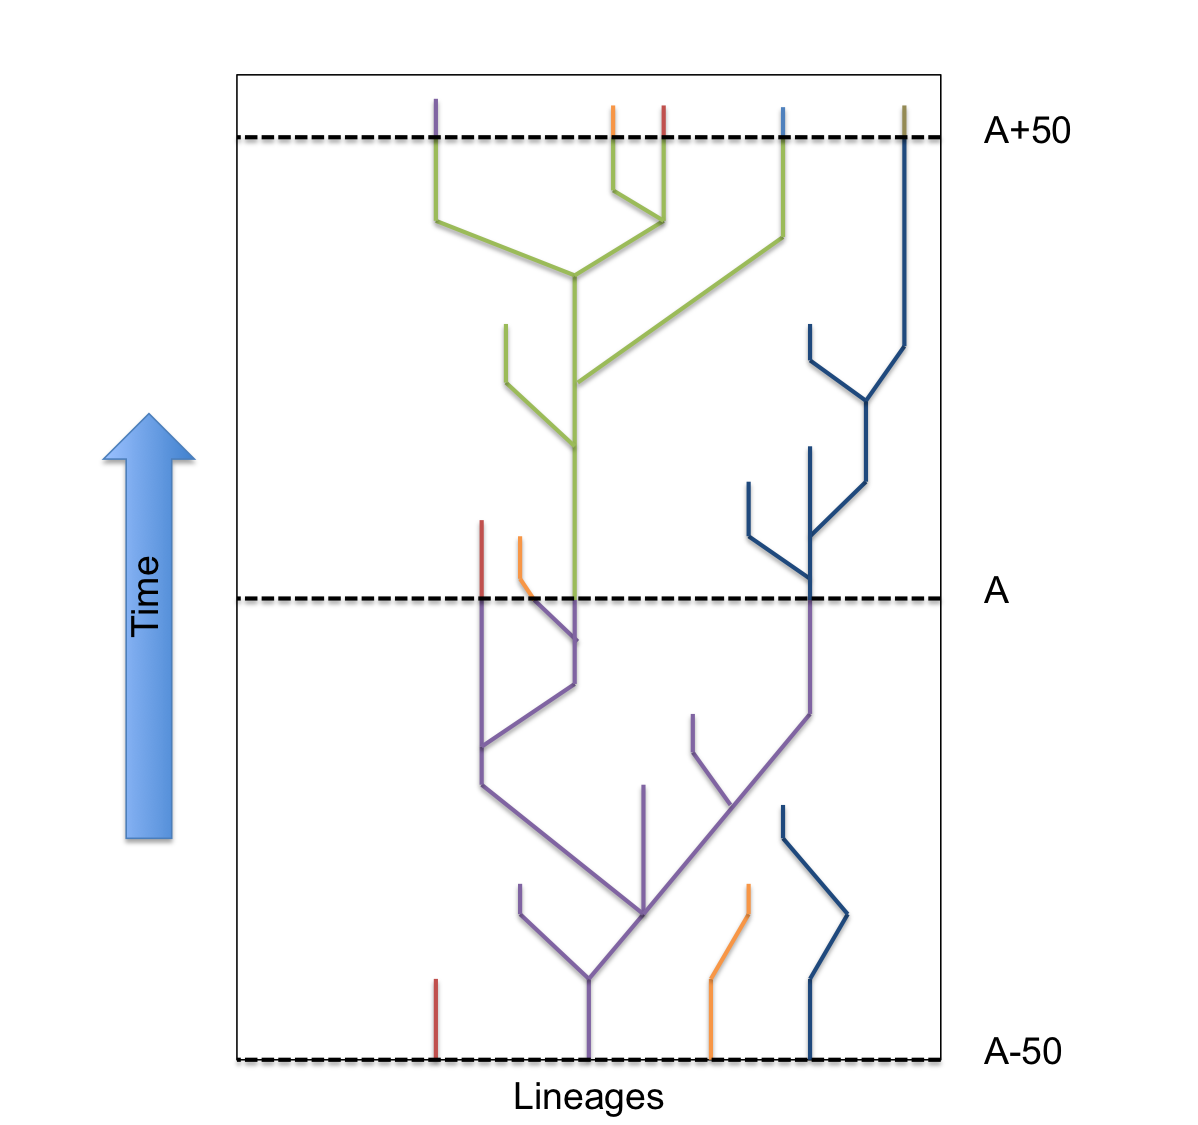
\includegraphics[width=3.5in]{figs/LineageFigure.png}
\caption{\textbf{An illustrative example of how we filter genomes for persistent lineages.} At time point A, the purple lineage has proven to be persistent and therefore the original genome from A-50 will be considered meaningful. Similarly, the green and blue lineages persist to time point A+50 and so the original green and blue genomes will be considered meaningful as they were at time point A.}
\label{lineages}
\end{figure}

\subsection{Informative Sites}
    While a genome may have descendants in 50 generations, this persistent genome may not be phenotypically different than another persistent genome in the population. To ensure we are not counting phenotypically identical genomes separately, we determine which sites in the genome contain information about the environment. In a an NK bitstring model, the only information that an organism can have about its environment is whether it is a better to have a 1 or a 0 at each site. Thus, informative sites are those for which flipping the corresponding bit would result in a fitness decrease. In calculating all of the following metrics, we first reduce the genome to its informative sites.
    This approach could easily be extended to any system in which the genome is made up of a sequence of elements that collectively determine fitness. The overall fitness effect of nullifying a given element in the genome is a decent proxy for the amount of information that site contained. A caveat to this technique is that genomes that achieve a given result in an excessively fragile manner may appear more complex than more robustly built genomes. To mitigate this issue, the combined fitness effect of eliminating multiple genome elements at once can be measured. Fortunately, this is not a risk in an NK model.

\section{Metrics}

\subsection{Change Metric}
    Our first metric focuses on whether the genetic makeup of the population is changing. This metric should always be above zero unless the population has converged and no beneficial variation is being introduced. We use our method of filtering genomes (explained previously) to ensure that we only record a genome as new compared to the previous time point if its lineage has persisted for one full time point. For this comparison, we first find the genomes from persistent lineages from time point A by determining which genomes have descendants in time point A + 50. In the example shown in Figure~\ref{lineages}, this would be the genomes at the root of the green and blue lineages. We then compare these genomes to those found to have been from persistent lineages in time point A-50 because they have descendants in time point A, purple in Figure~\ref{lineages}. In this way, we create a sliding window to observe change in the population.

\subsection{Novelty Metric}
    The novelty metric measures how many genomes have evolved in the population that have never been seen previously in the experiment. For this metric we again filter out genomes that do not have descendants in the next time point, enabling us to focus on meaningful novelty. To measure novelty, we simply count how many genomes from persistent lineages (genomes that existed in time point A and have descendants in time point A+50) have never been in a previous time point’s persistent genome pool. It is possible with this metric for a genome to evolve, but not persist, and therefore not be recorded in the permanent history, but then evolve and persist at a later point and be counted as novel. Once a genome has been counted as novel, however, it is part of the permanent history and will never be counted in the novelty metric again. Thus, while a genome could be delayed in being counted as novel, it will not be counted twice.
    

\subsection{Complexity Metric}
    The complexity metric measures if the complexity of the population is increasing. To determine if the complexity is increasing, we only need to focus on the most complex organism in the population at a given time point. We are considering complexity in the information theory sense of the term, and therefore focusing on only informative sites in an organism’s genome. Because the ones of an organism’s genome are the sites that contribute to its fitness, we determine an organism’s complexity by how many ones it has in its genome. Therefore, our complexity measure is simply how many bits are ones in the organism with the most ones in its genome. In our simple simulation, the number of ones is under selection and therefore should increase until all organisms have all ones in their genome. Therefore, the complexity metric cannot increase indefinitely in our simulation, but will demonstrate what can be expected in a closed evolutionary system.

\subsection{Ecological Metric}
    The ecological metric measures the amount of information in the population as a whole. While individuals may not contain increasing amounts of information in single genomes (as measured by the complexity metric), they could still be increasingly diverse and therefore contain increased information collectively in the population. We can measure such a phenomenon by looking at the diversity of persistent genotypes reduced to informative sites. Complex ecologies in which multiple subsets of the population are using different information about the environment to survive are likely to be characterized by a relatively balanced distribution of individuals across the various successful phenotypes. Thus, we use Shannon entropy, a popular metric of diversity that also measures evenness, to measure the diversity of the persistent genotypes and calculate the ecological metric.



\section{Results}
    To ensure that these metrics are capturing the dynamics that we want them to, we tested them on a range of variants on our basic NK model, described above.  The preliminary results for each metric are described below.

\subsection{Change Metric}
For a system to exhibit open-ended evolution, it is clearly necessary for it to be changing by producing genomes meaningfully different from a previous population, though not necessarily completely novel. Therefore, we first measured the meaningful change of our system under varying environmental conditions to demonstrate how differing environments can differ in even this simple metric. As shown in Figure~\ref{change_time}, several environmental changes increase the amount of meaningful change found in the populations over time. When organisms are forced to share fitness between others with the same genotype, the amount of change increases and remains higher than the baseline over time. Conversely, when the environment changes frequently, there is an initial spike of increased change that quickly drops back down to the baseline value.

\begin{figure}
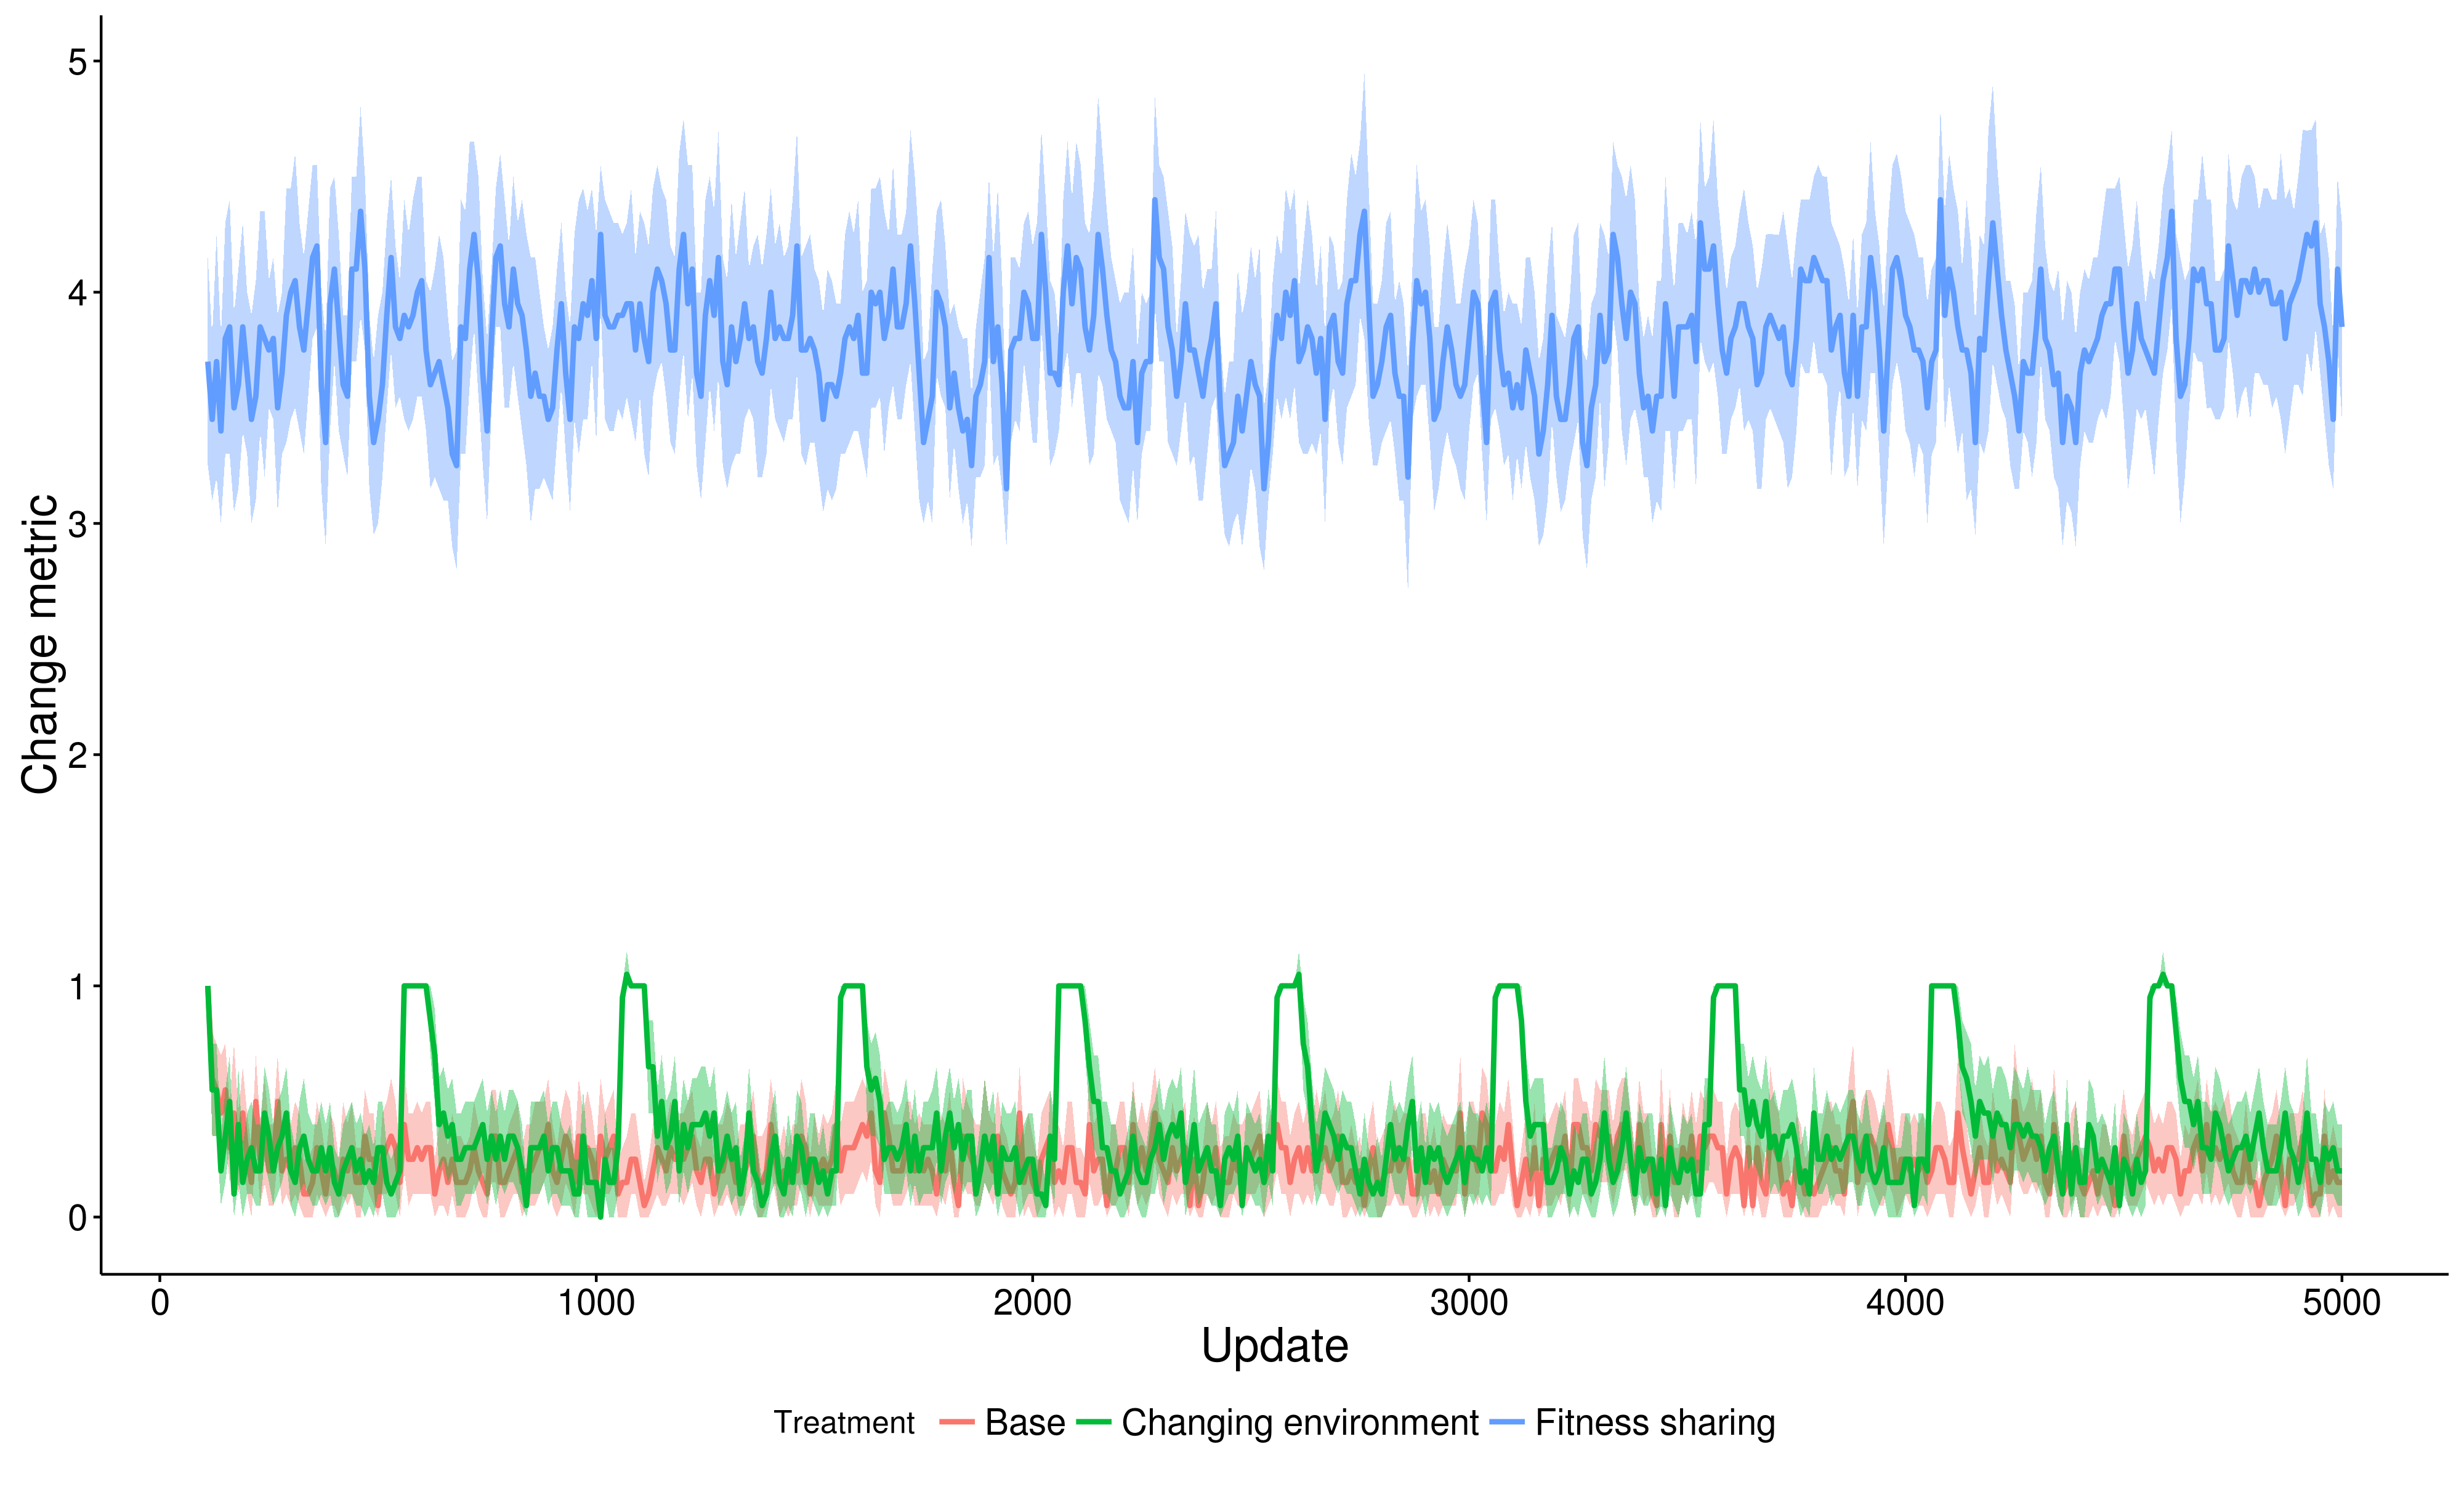
\includegraphics[width=3.5in]{figs/change_changing_environments.png}
\caption{\textbf{Amount of change at over time in varying environments.} As measured by the change metric, fitness sharing increases the amount of change in the population over time. Conversely, a routinely changing environment leads to spikes in change that quickly drop as the population converges again.}
\label{change_time}
\end{figure}

The majority of environmental conditions we tested produced dynamics over time qualitatively similar to the baseline treatment. Therefore in Figure~\ref{change} we show the amount of meaningful change in populations at the final time point in more environmental conditions. Larger genomes (N) lead to increased meaningful change because they allow for a larger search space that the population can continuously mutate within, leading to more beneficial mutants. A higher mutation rate leads to increased meaningful change because mutations are necessary to create any meaningful change in our system. A smaller population size produces more meaningful change because a small population cannot hold as many different genomes at one time and therefore there are more genomes that can arise that are different than what is in the previous population. Finally, fitness sharing can produce increased meaningful change because it favors new phenotypes that do not have to share fitness, making them more likely to persist.

\begin{figure}
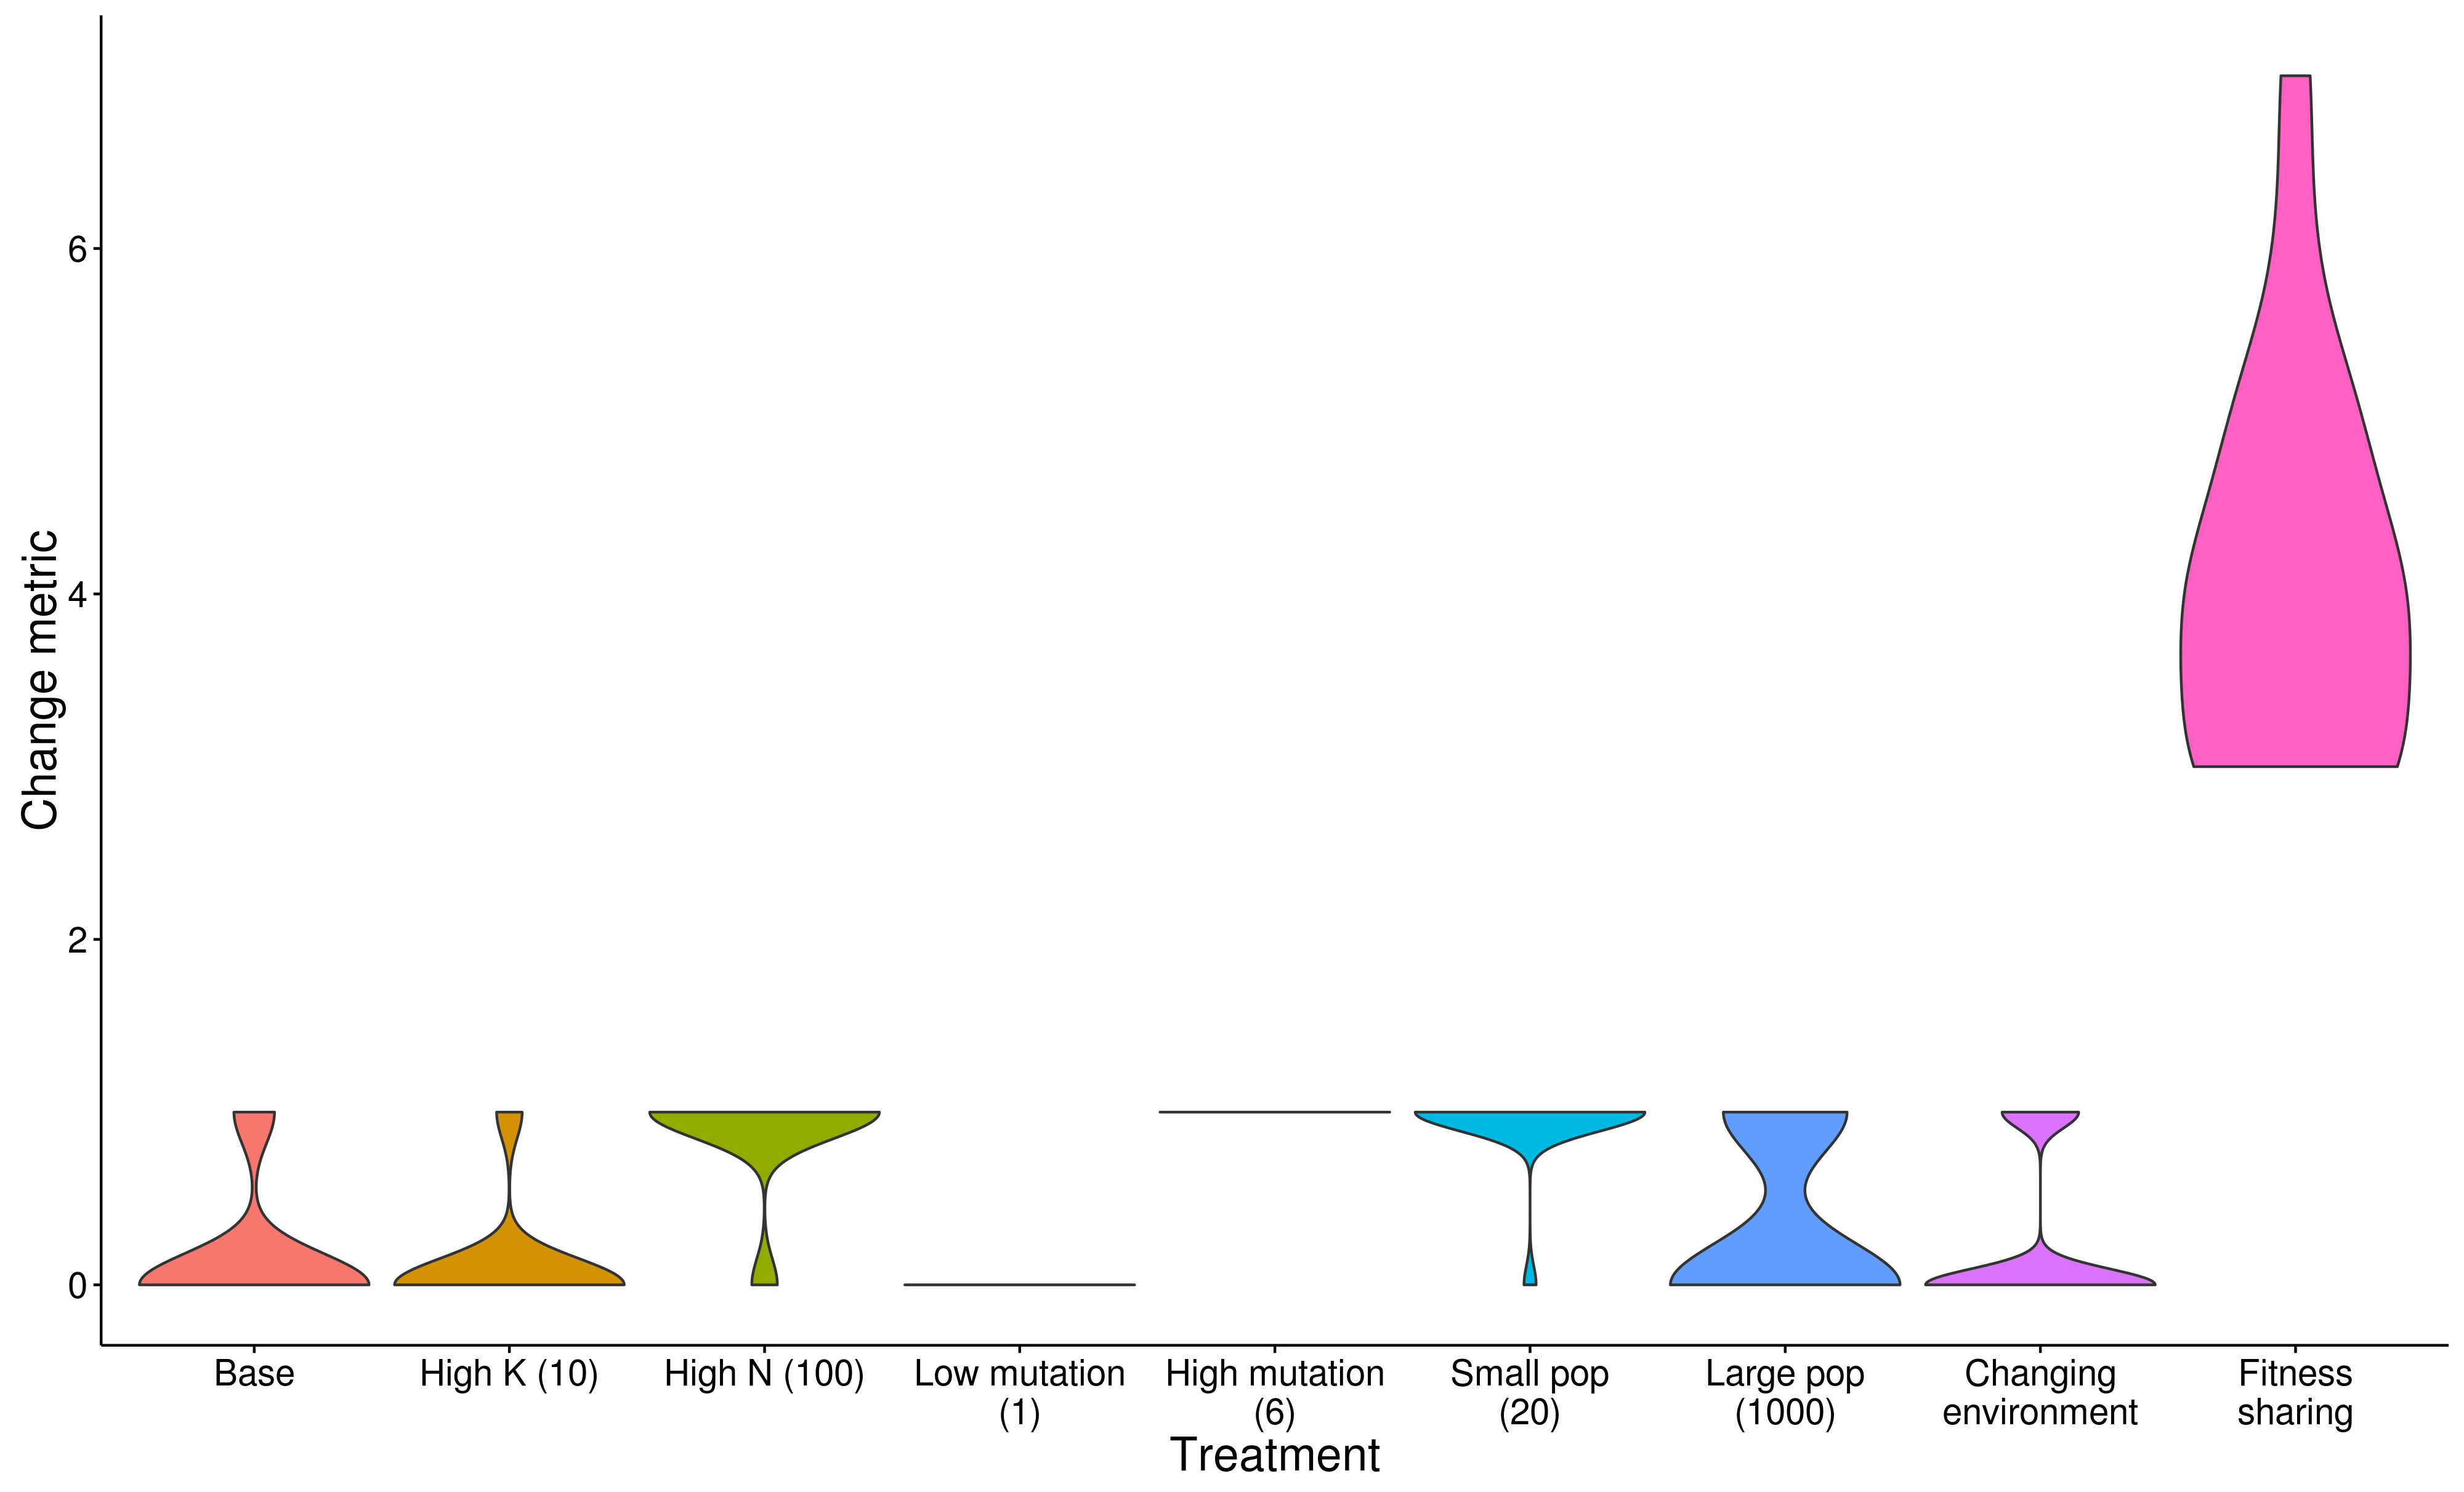
\includegraphics[width=3.5in]{figs/changeboxplots.png}
\caption{\textbf{Amount of change at final update in varying environments.} As measured by the change metric, environmental conditions that increase the amount of change at the final time point include: increasing the size of the genome (N), increasing the mutation rate, decreasing the population size, and implementing fitness sharing.}
\label{change}
\end{figure}

These results show that while change is a metric often not considered in discussions of open-ended evolution, the amount of meaningful change can reflect differences in the environment and evolution of the populations and is likely a necessary dynamic for open-ended evolution.

\subsection{Novelty Metric}
The continuous production of meaningfully new genomes is necessary for what is generally considered open-ended evolution, because without meaningfully novel genomes, nothing `interesting' can emerge. Therefore, our second metric measures the amount of meaningfully novel genomes (i.e., have never been recorded previously) that have persisted in a population since the previous time point. As shown in Fig~\ref{novelty_time}, the a higher mutation rate increases the amount of novelty measured by our metric. This result is because more mutations make it more likely that more meaningful mutants will arise and therefore that more completely novel mutants will emerge. As expected, even at a high mutation rate, novelty does start to decrease over time as the search space is explored.

\begin{figure}
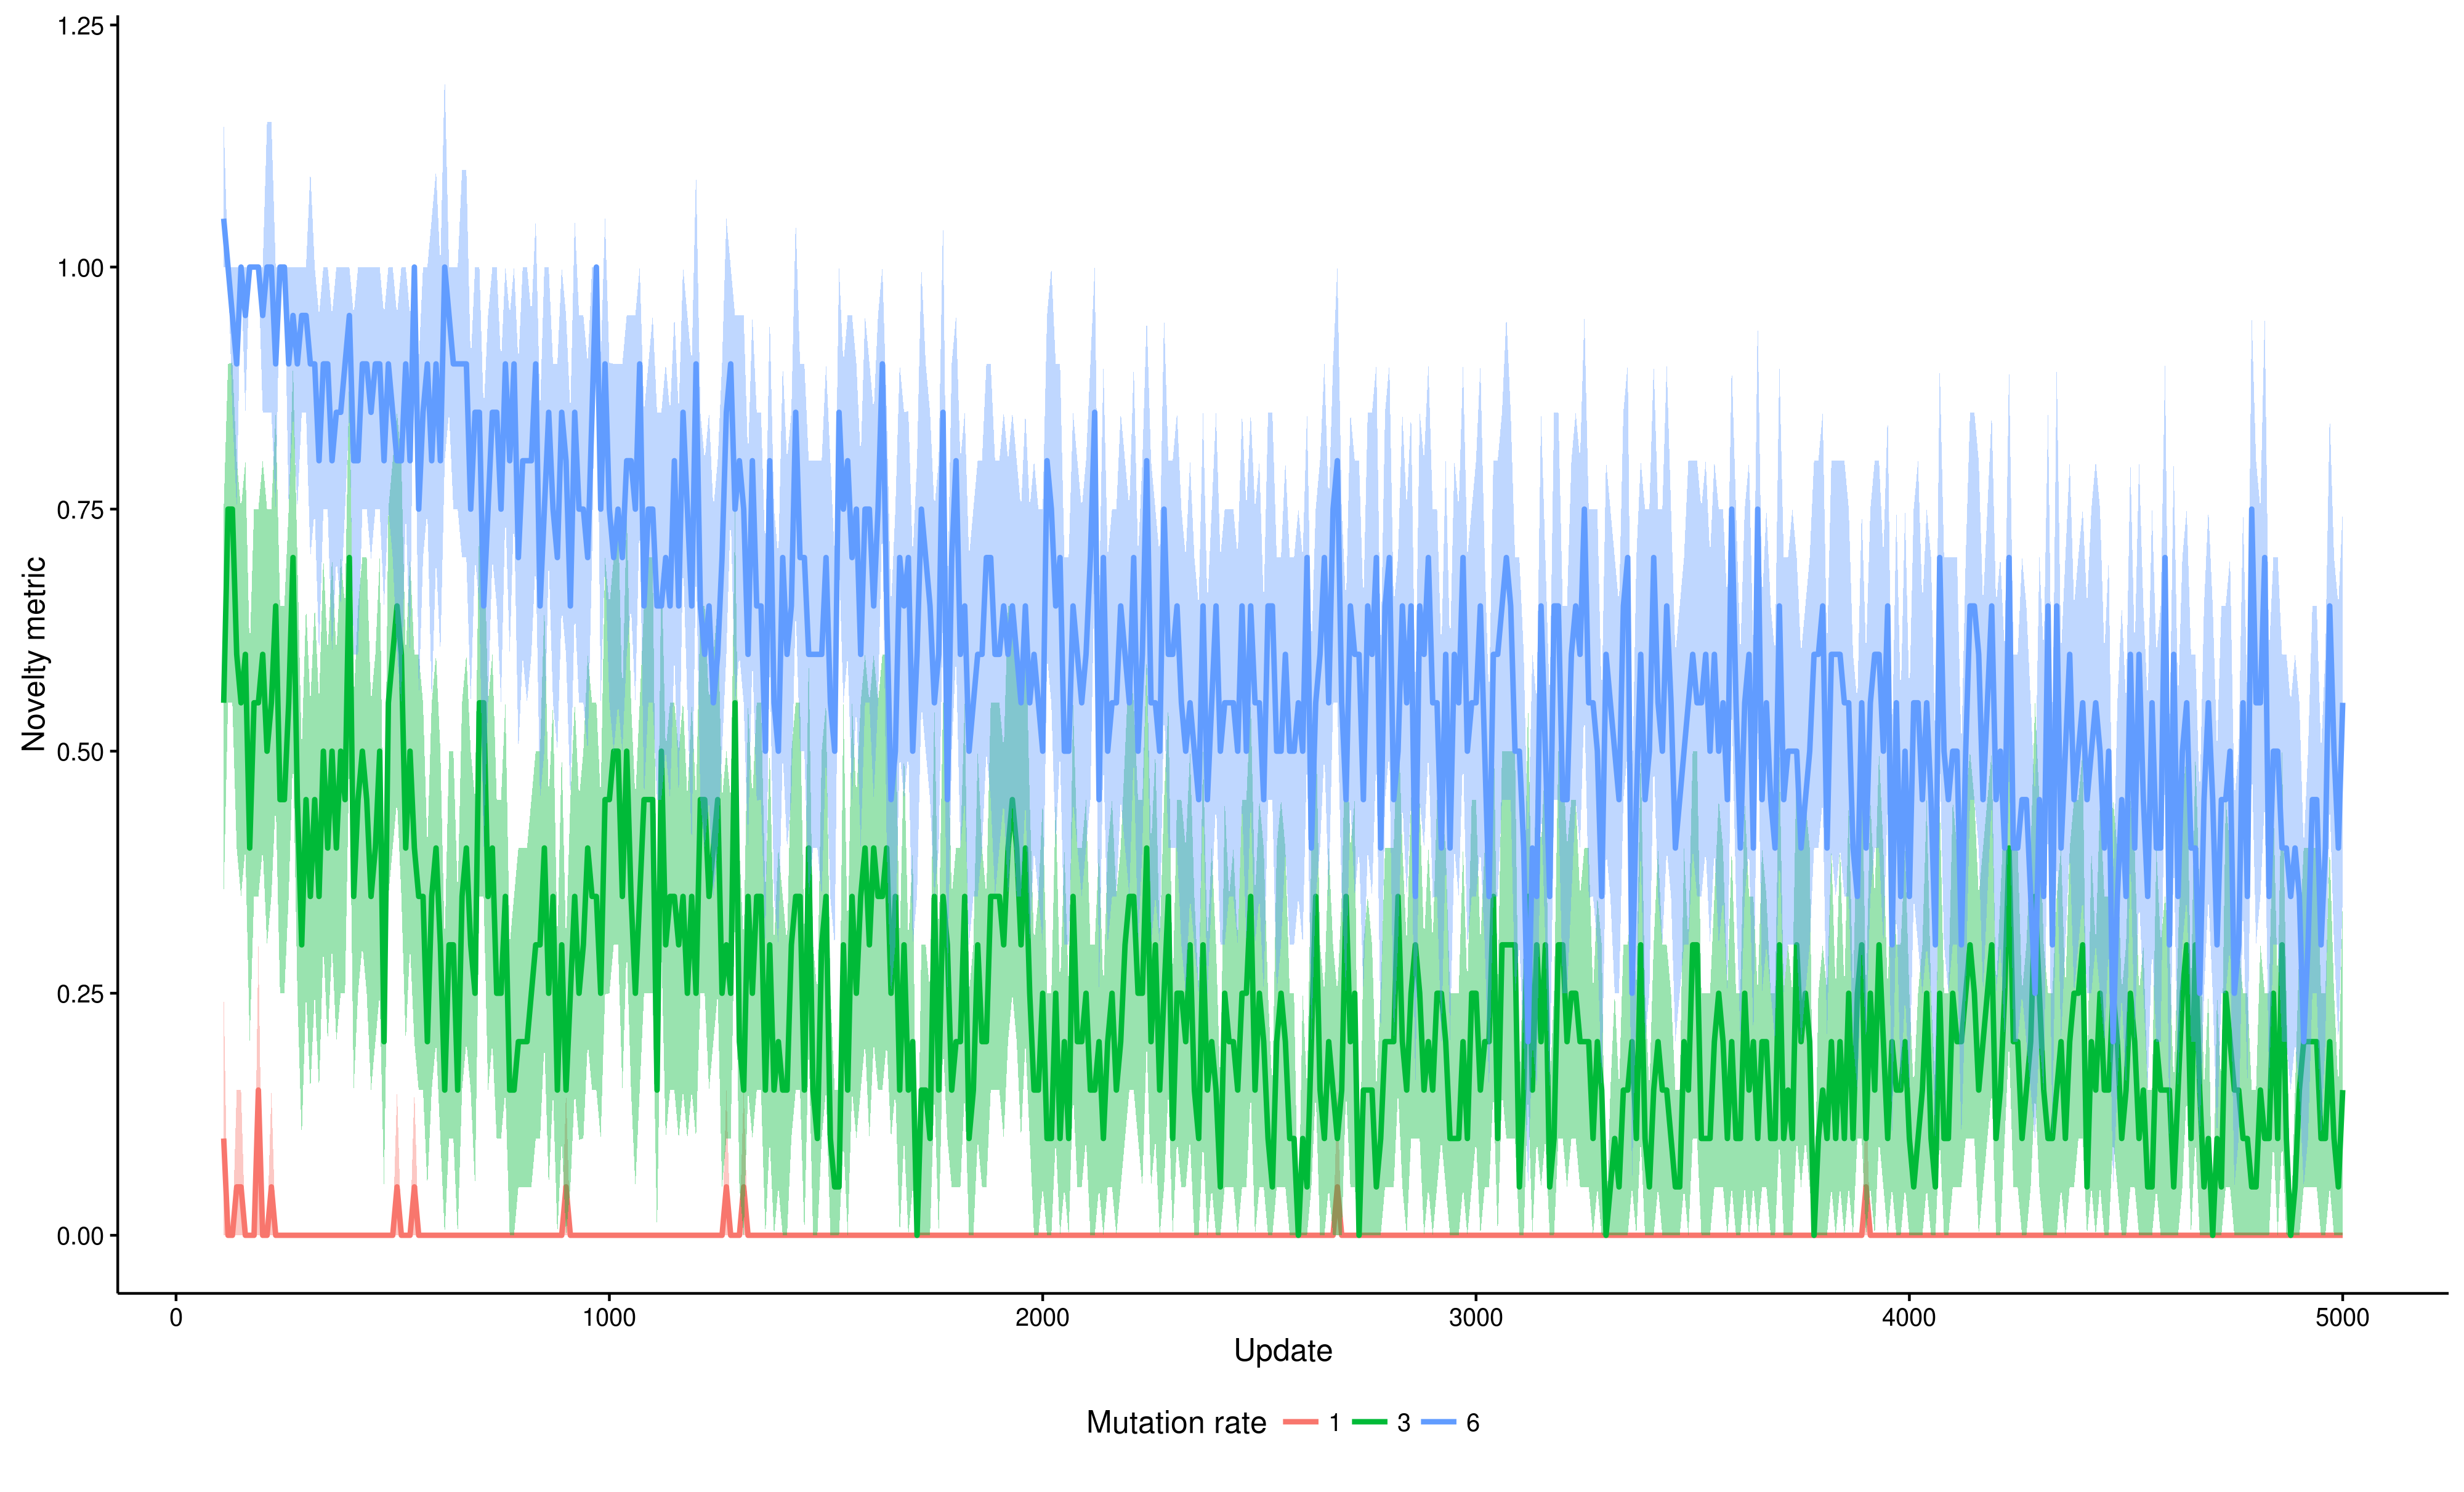
\includegraphics[width=3.5in]{figs/novelty_mean_mut_rate.png}
\caption{\textbf{Amount of novelty over time with varying mutation rate.} The novelty metric measures the number of completely new meaningful genomes that have lineages that persisted since the previous time point. As the mutation rate increases, more novelty is continuously produced, however at all mutation rates, the novelty decreases over time. Mutation rate 3 is the baseline treatment in previous graphs.}
\label{novelty_time}
\end{figure}

We again found that the majority of treatments had a qualitatively similar trajectory over time and therefore in Figure~\ref{novelty} we show only the final novelty value. As predicted, the baseline treatment does not produce any meaningful novelty by the final time point. However, many environments do allow for continuing production of novelty, specifically epistasis (K), larger genomes (N), higher mutation rate, differing population size, and fitness sharing. Epistasis increases novelty produced in the final update because the population must explore a rugged fitness landscape instead of converging to a single fitness peak, leading to more novel genomes to discover throughout evolution. Larger genomes allow for more novelty at the final update because they increase the size of the search space and therefore how many genomes can ever be considered novel. Smaller population sizes increase novelty at the final update because it takes the population longer to discover many genomes, leaving enough to still be novel at the end of the experiment. Conversely, larger population sizes allow for some increase in novelty over the baseline treatment because the increased number of organisms makes it easier for more of the search space to be explored. Finally, fitness sharing increases the final novelty by selecting for novel genotypes because a novel genotype will not have to share its fitness and therefore be more likely to persist.

\begin{figure}
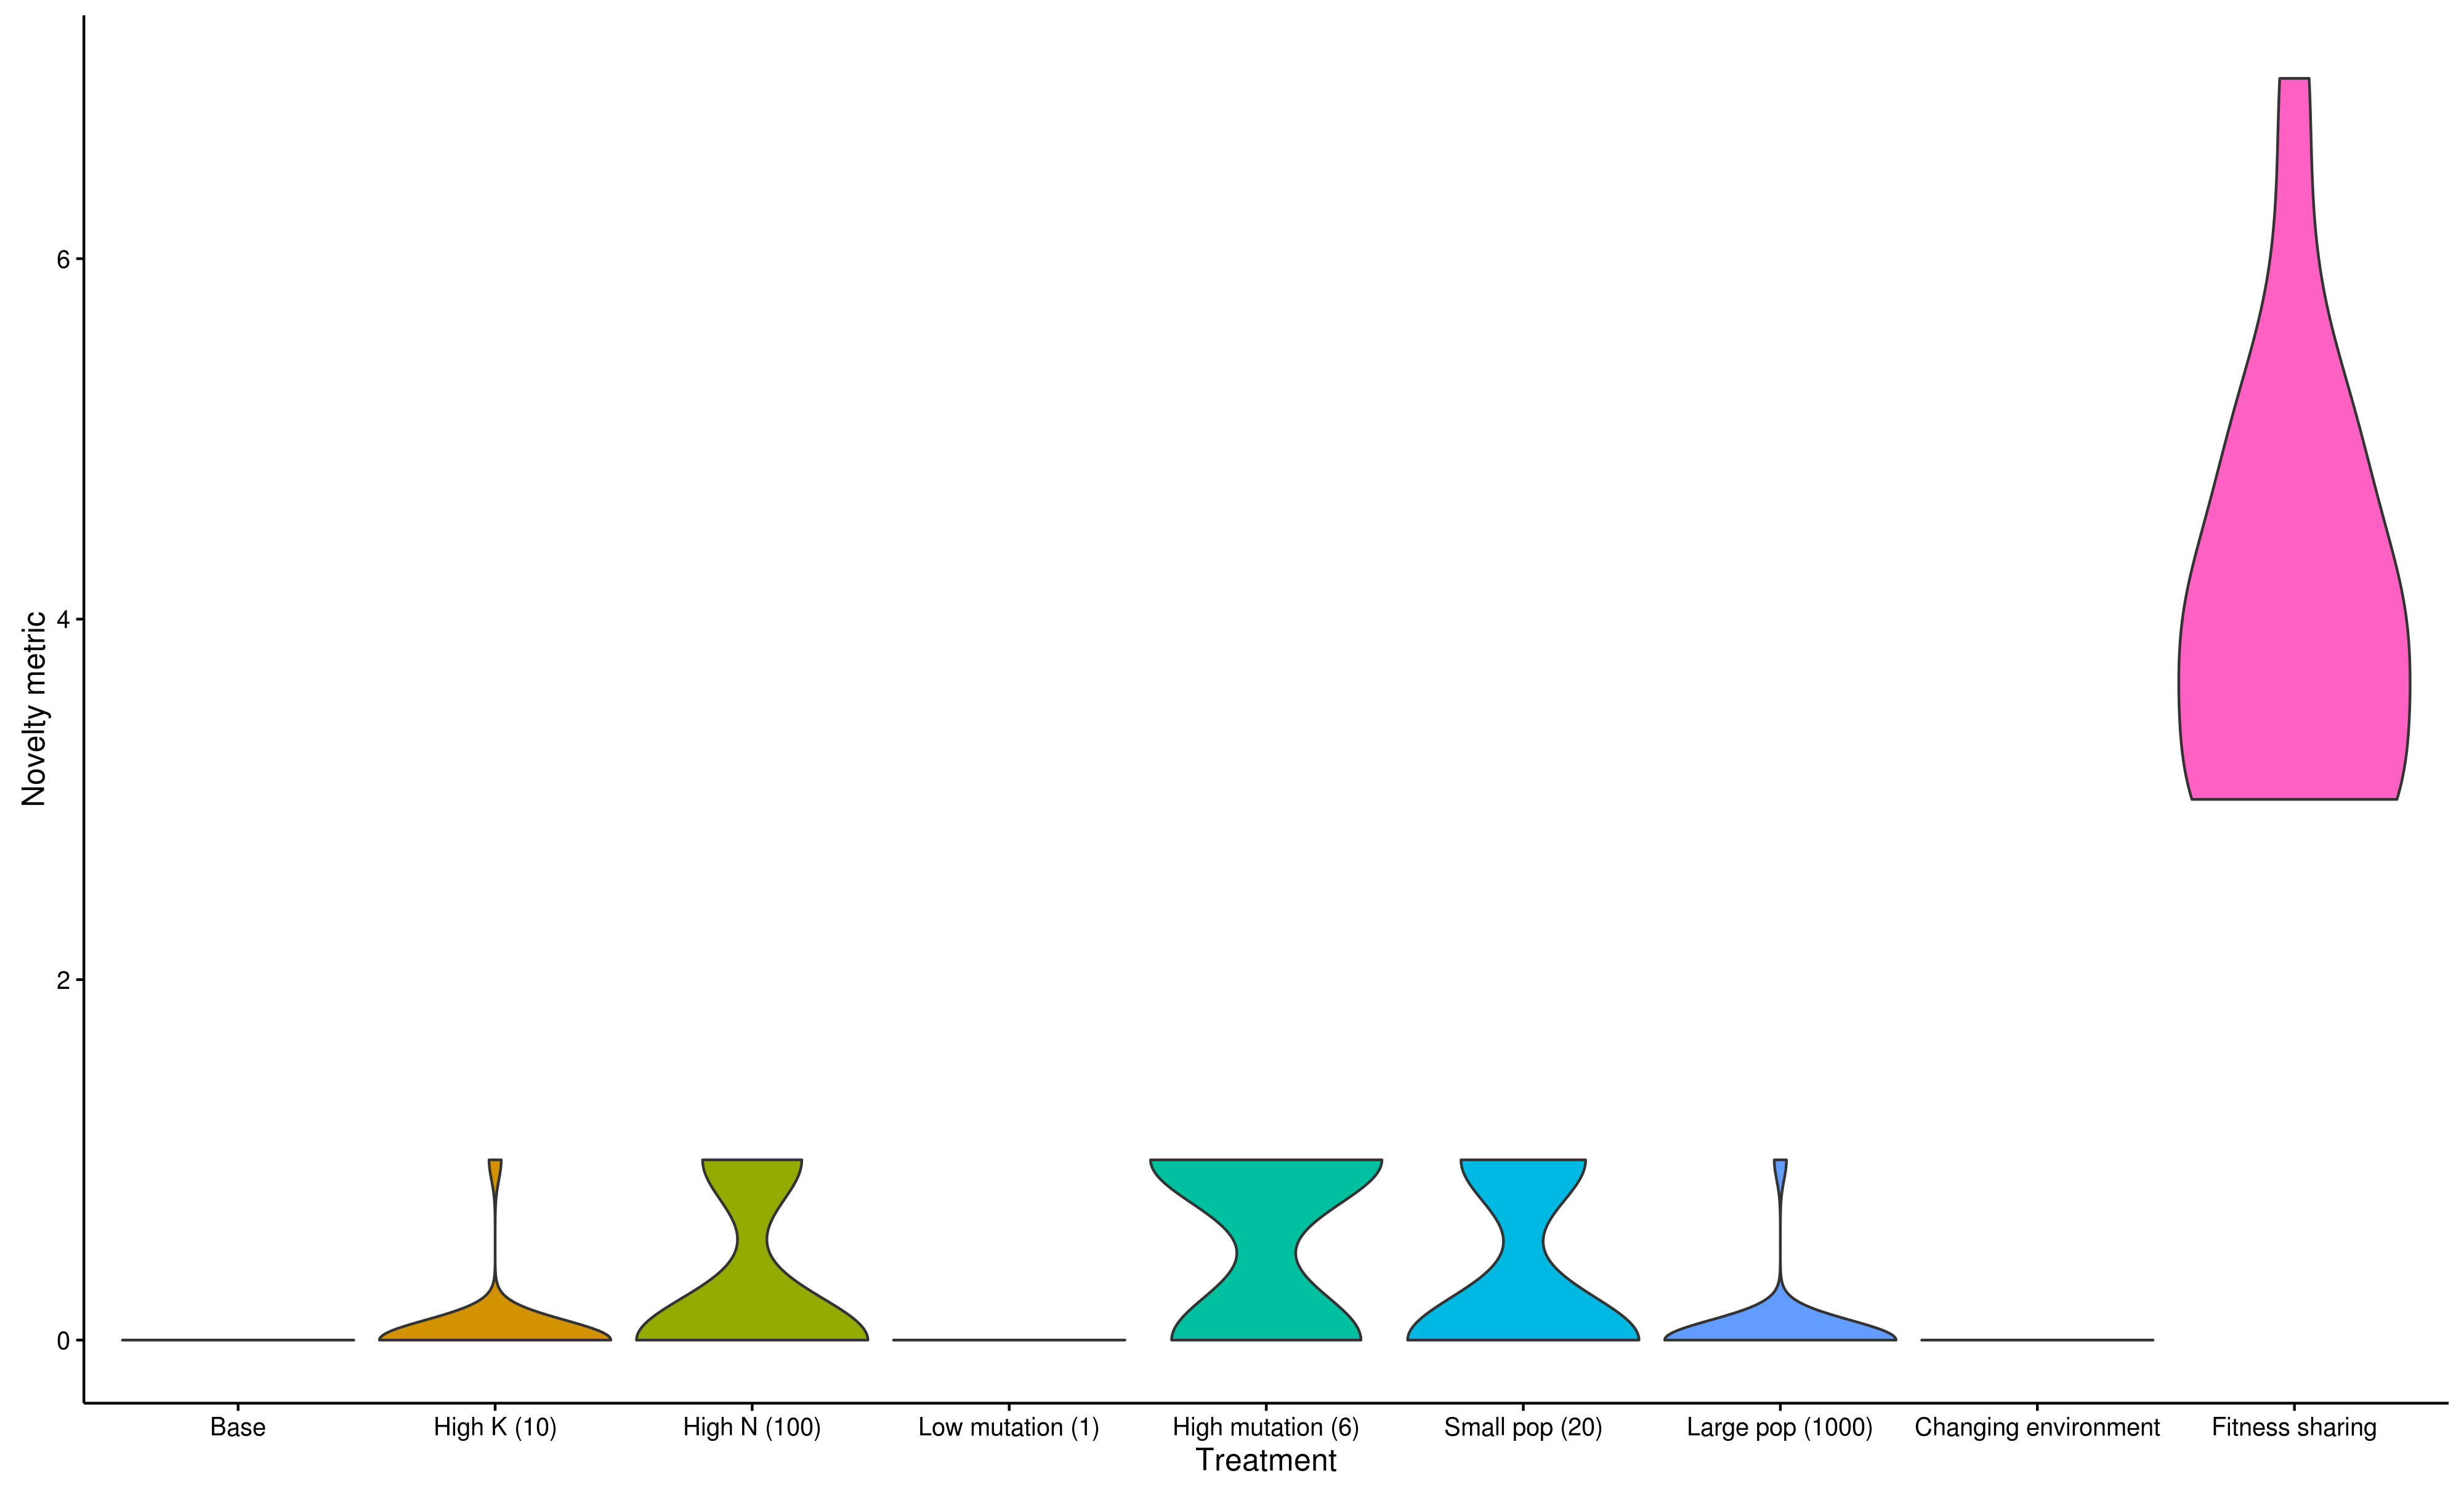
\includegraphics[width=3.5in]{figs/noveltyboxplots.png}
\caption{\textbf{Amount of novelty at final time point in varying environments.} At the final time point, no meaningful novelty is found in our baseline populations. However, increasing the amount of epistasis (K), increasing genome length (N), increasing mutation rate, decreasing population size, and enabling fitness sharing increase the amount of novelty produced in the final time point.}
\label{novelty}
\end{figure}

These results highlight the power of the novelty metric to identify environments and populations that have the potential to be open-ended due to the high amount of new genotypes being consistently discovered. Novelty is likely necessary, but not sufficient, for open-ended evolution because if nothing new is being produced by a population, neither the complexity nor the ecological metric can be non-zero.

\subsection{Complexity Metric}
    An ideal open-ended evolutionary system would likely have increasingly complex individual organisms. Therefore, we next compared our complexity metric between different environmental conditions in our model. We calculated the complexity of the most complex organism of each population over time, as Figure~\ref{complexity_time} shows. We found that in our baseline treatment, there is a limit to how complex the organisms can evolve to be and therefore over time the complexity increases and then saturates. Conversely, fitness sharing leads to lower complexity because it weakens selection for climbing fitness peaks if there is a large amount of the population on the same fitness peak.

\begin{figure}
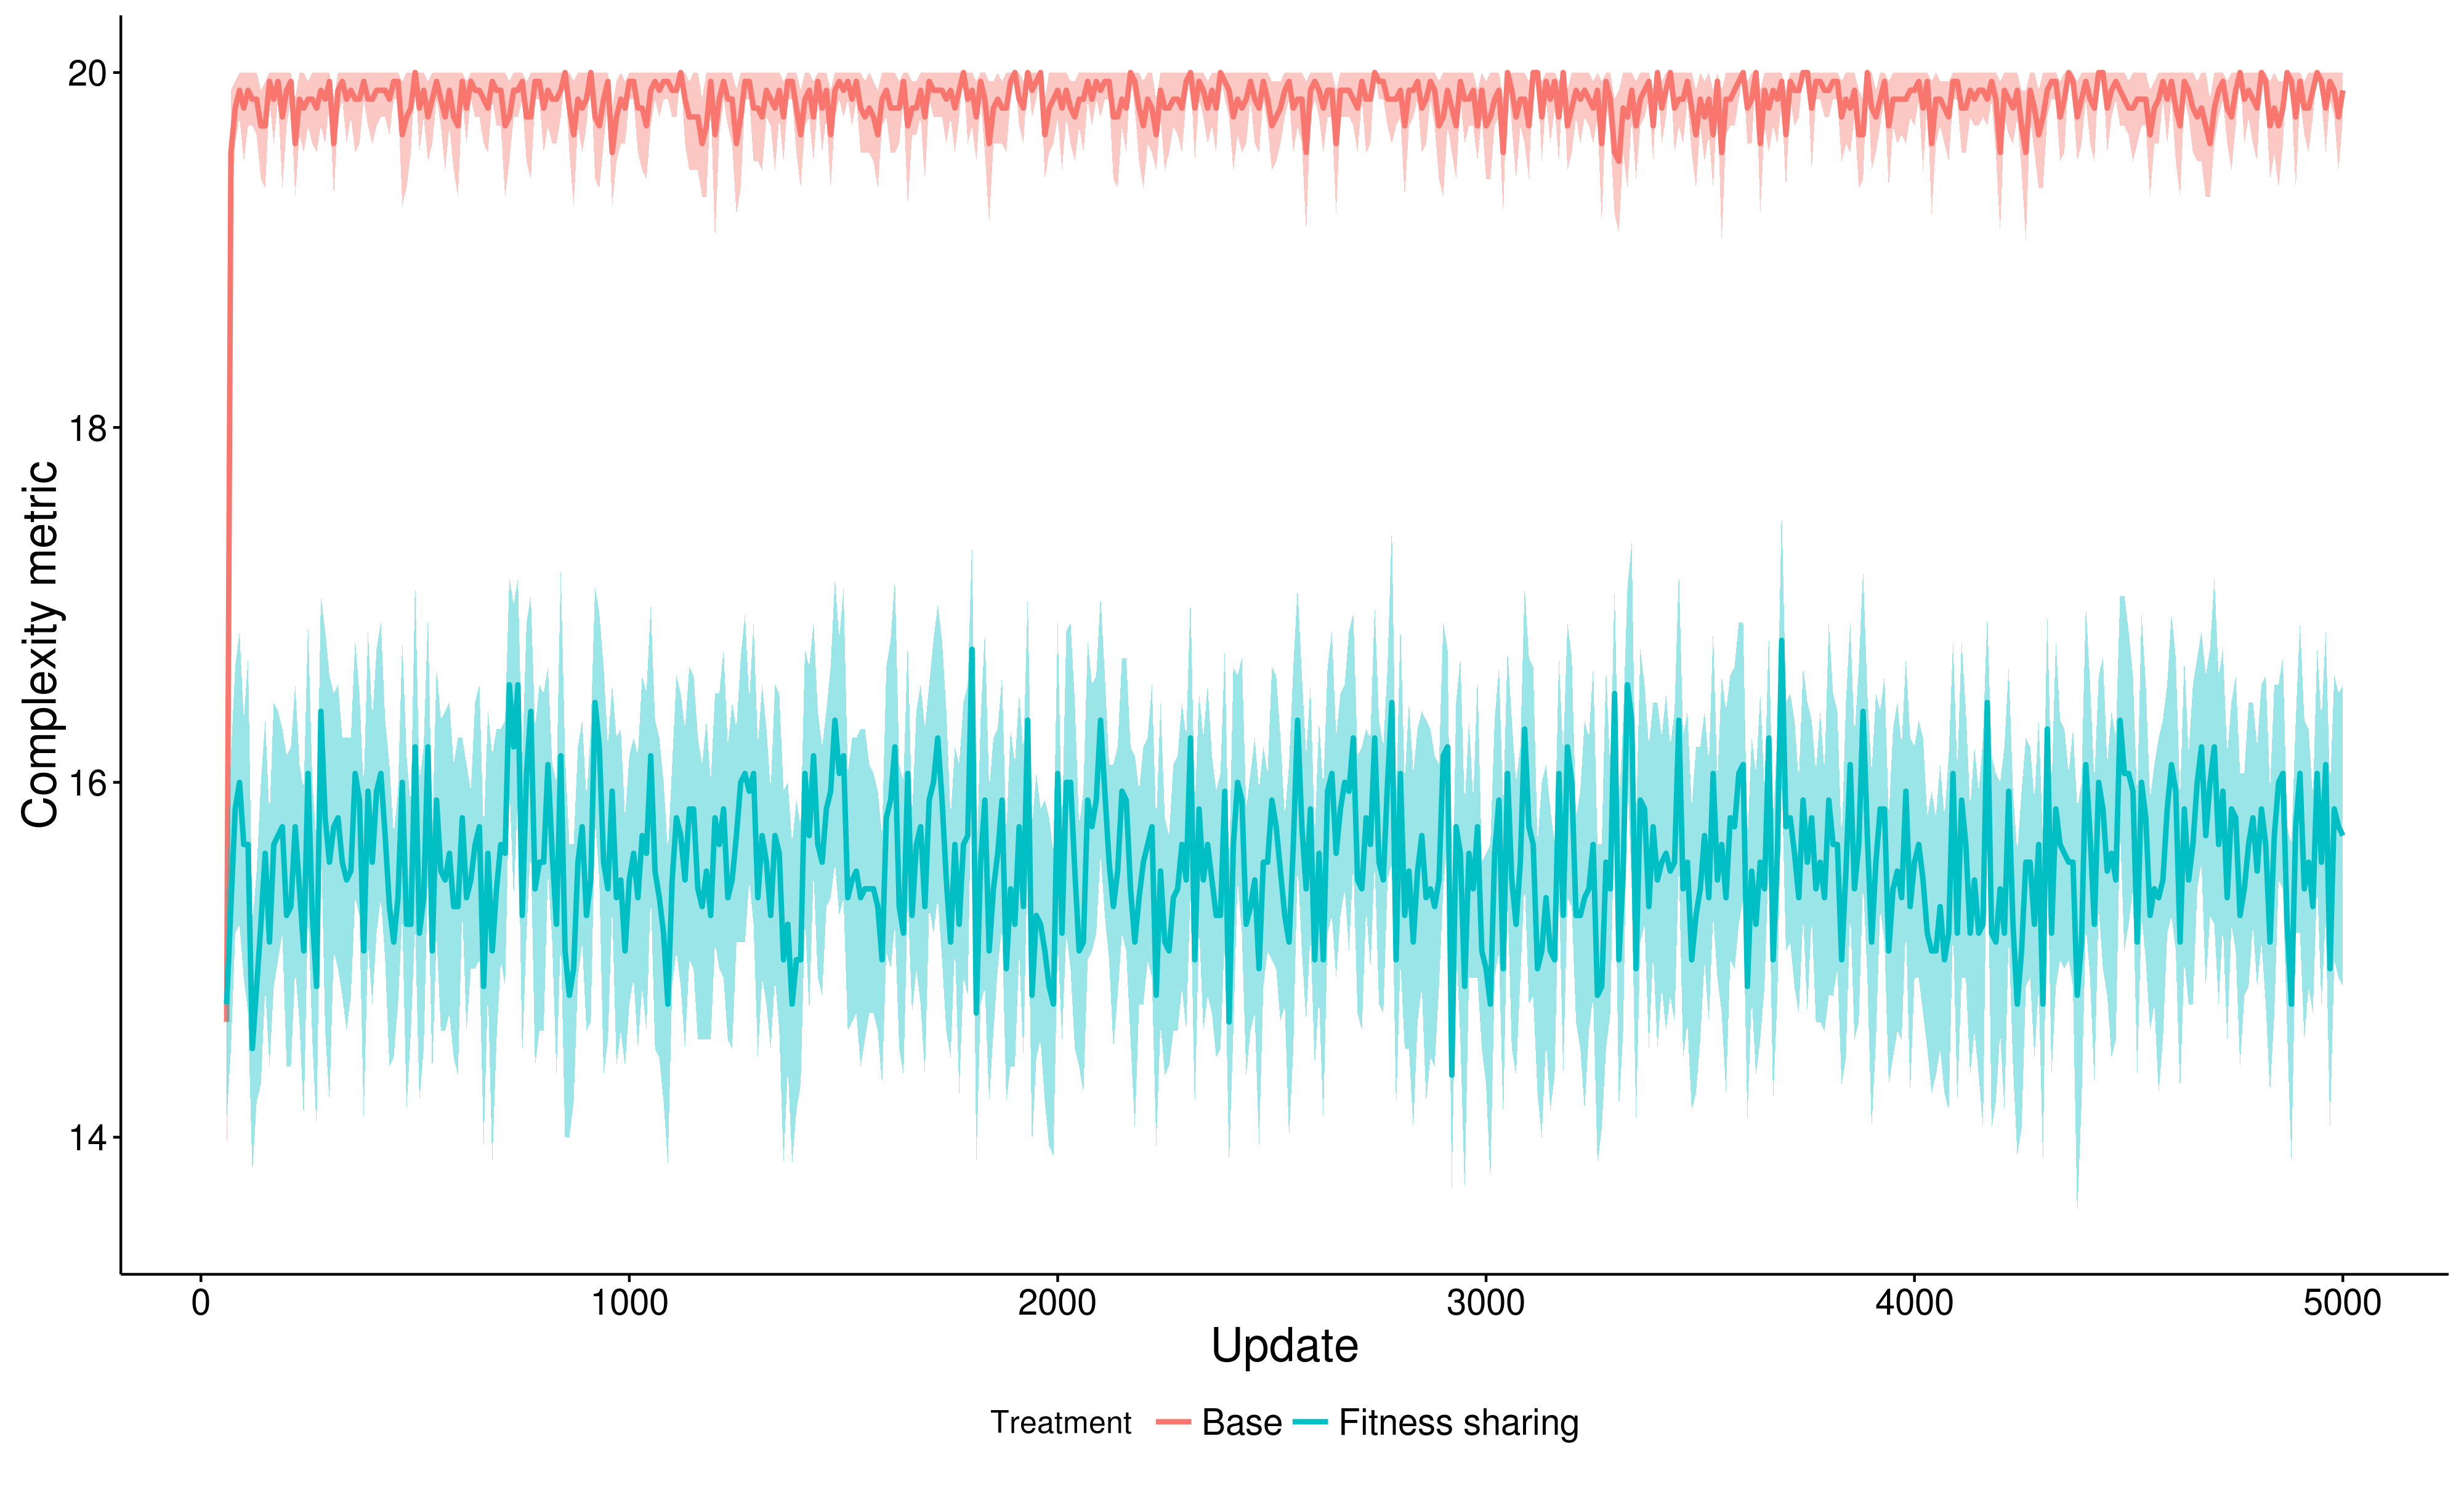
\includegraphics[width=3.5in]{figs/complexity_fitness_sharing.png}
\caption{\textbf{Amount of complexity over time with fitness sharing.} The baseline treatment (red) is able to reach the top complexity allowed by the model quickly and remain at that value. When fitness sharing is introduced (blue), the population is not able to attain the top complexity value.}
\label{complexity_time}
\end{figure}

Because of the simplicity of our system, the complexity metric stabilizes quickly in most treatment and therefore we show only the final time point value for complexity in Figure~\ref{complexity}. The baseline treatment was able to reach the maximum complexity possible for a 20-bit genome and most of the environments did not decrease in the final complexity value. When the genome length was increased to 100 bits, the populations were able to reach the new maximum complexity value of 100. However, high mutation rate, smaller population size, and fitness sharing all somewhat decreased the final complexity achieved on average. A high mutation rate decreased the final complexity because it introduces more deleterious mutations and therefore slows adaptive evolution. A smaller population size decreased the complexity somewhat becaus

\begin{figure}
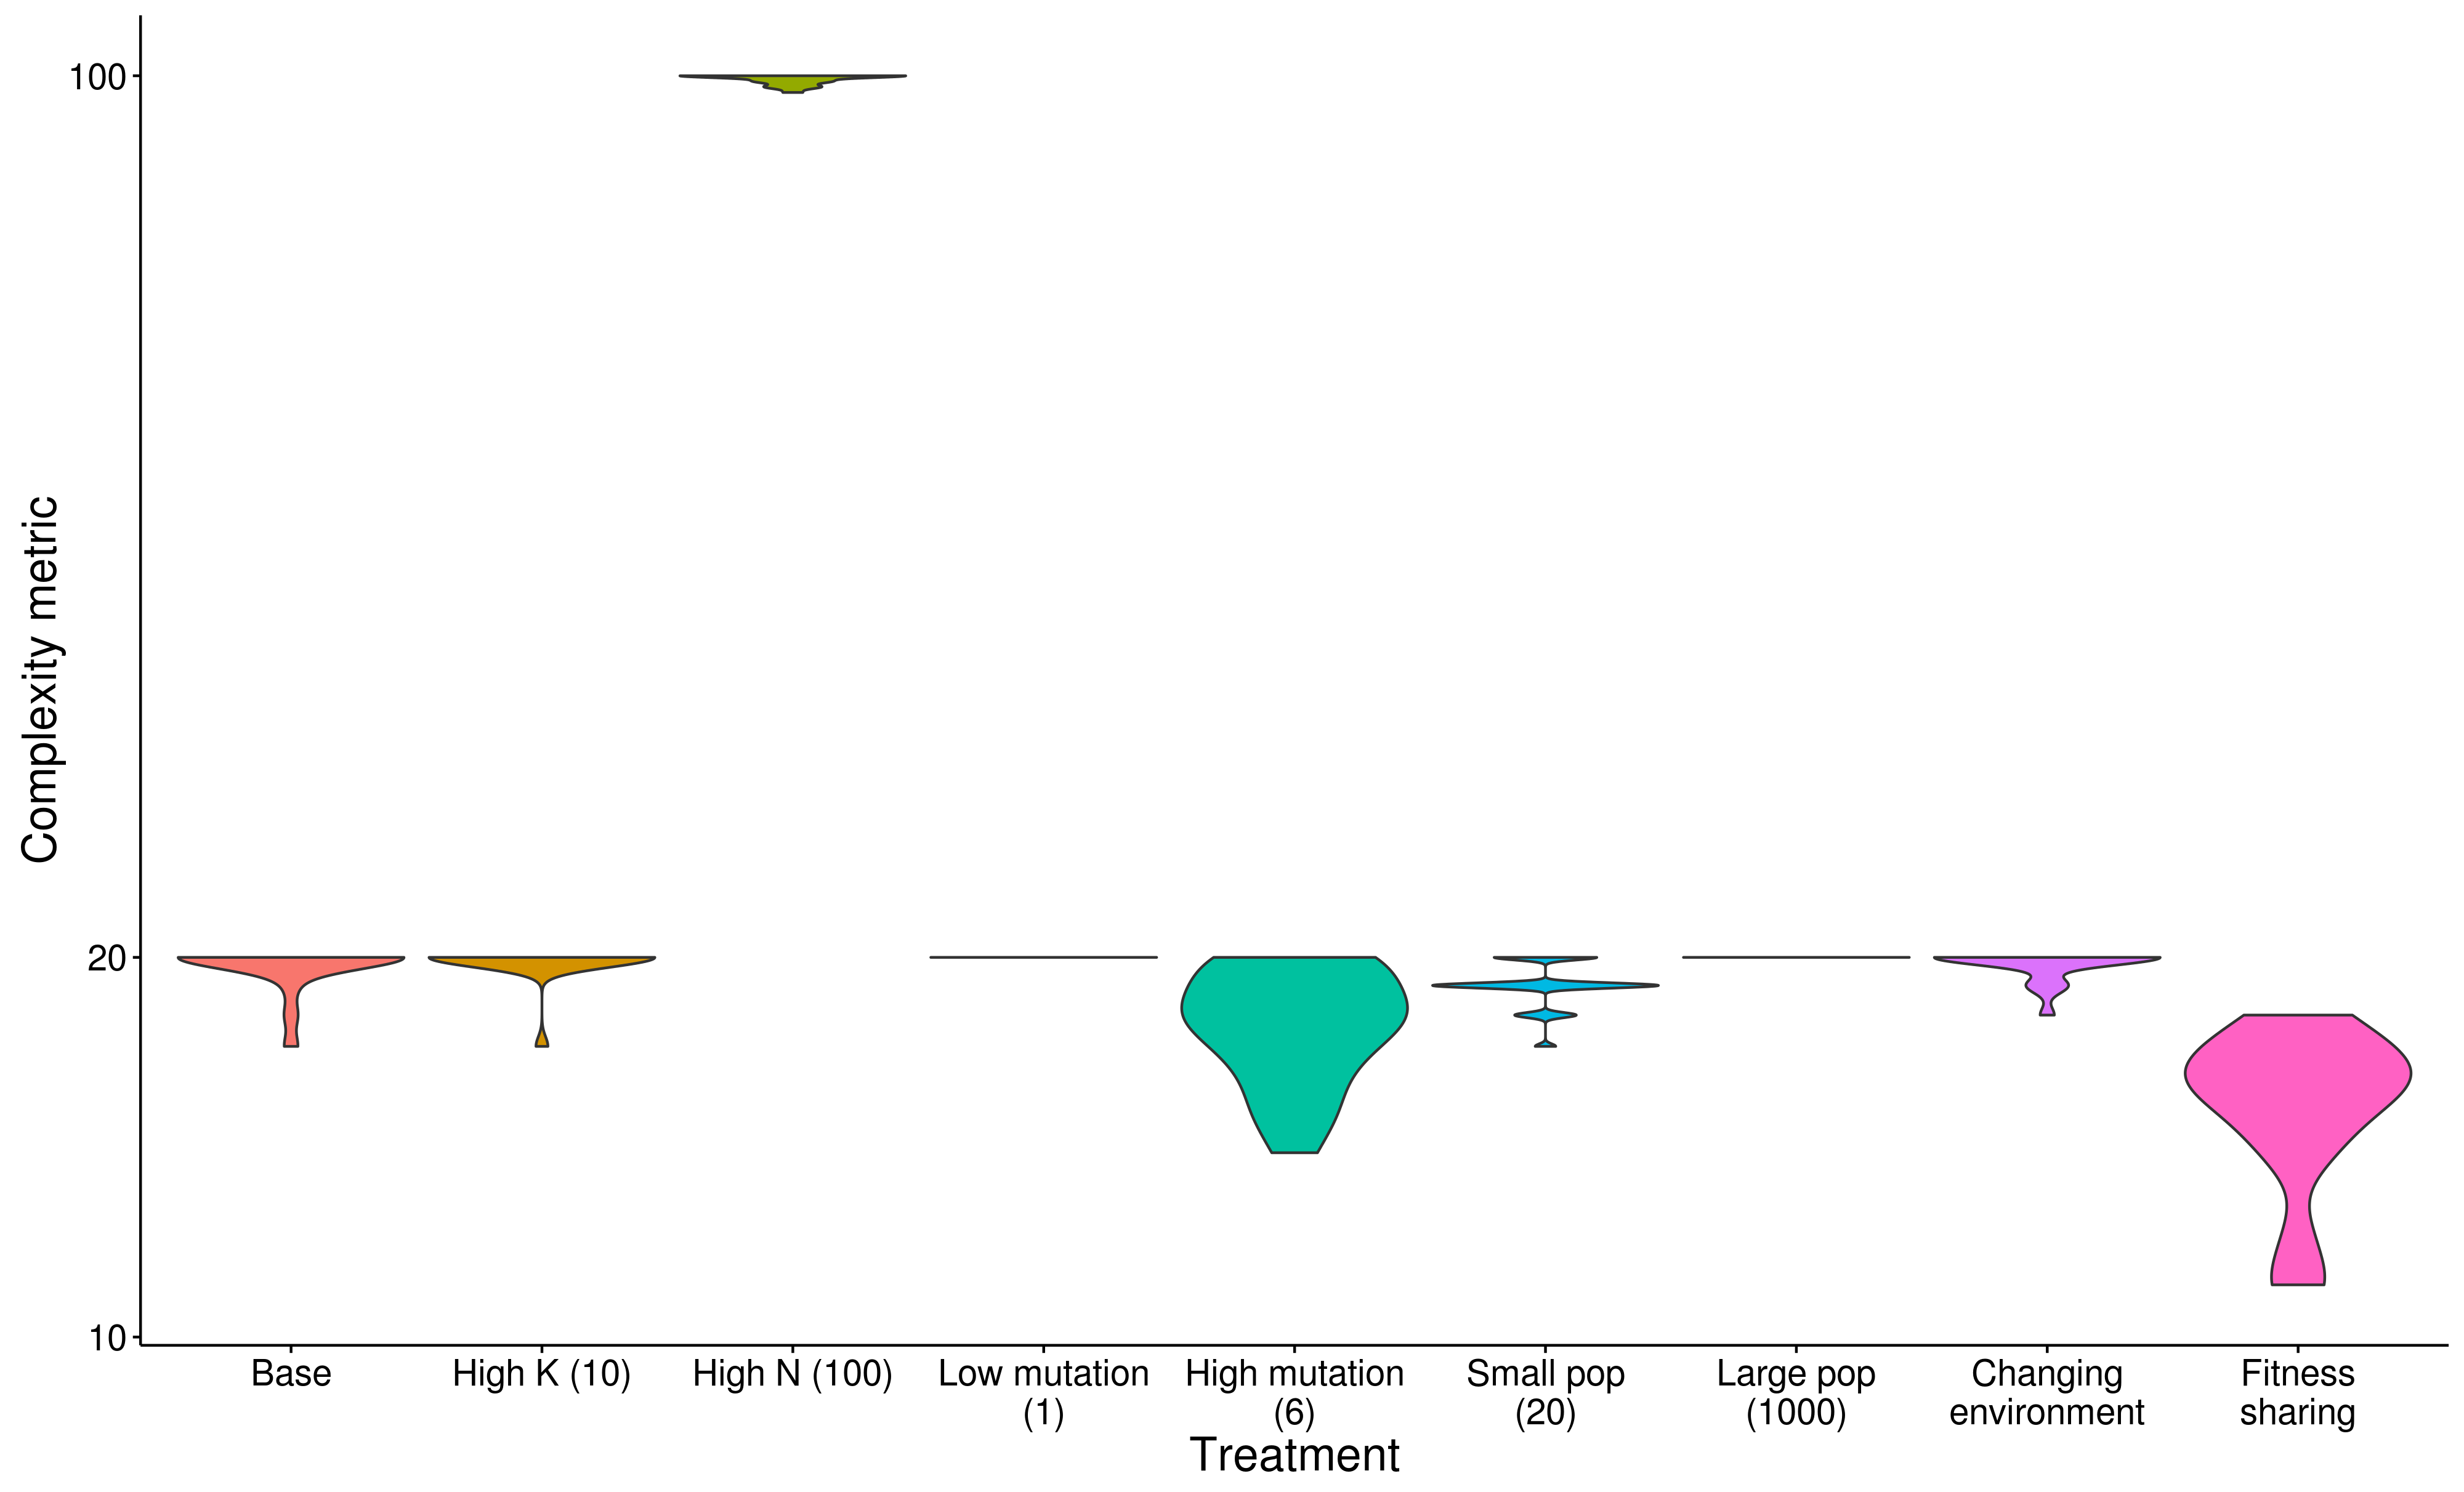
\includegraphics[width=3.5in]{figs/complexityboxplots.png}
\caption{\textbf{Amount of complexity at final time point in varying environments.} }
\label{complexity}
\end{figure}

\subsection{Ecological Metric}
Finally, an open-ended evolutionary system should not only have individually complex organisms, but a diverse population of interacting organisms. Even if a system is not evolving more complex individual organisms, it may still be exhibiting interesting dynamics because it allows for a large number of niches and therefore diverse organisms to occupy those niches. Our ecological metric captures this dimension of open-ended evolution. The ecological metric shown in Figure 5 

\begin{figure}
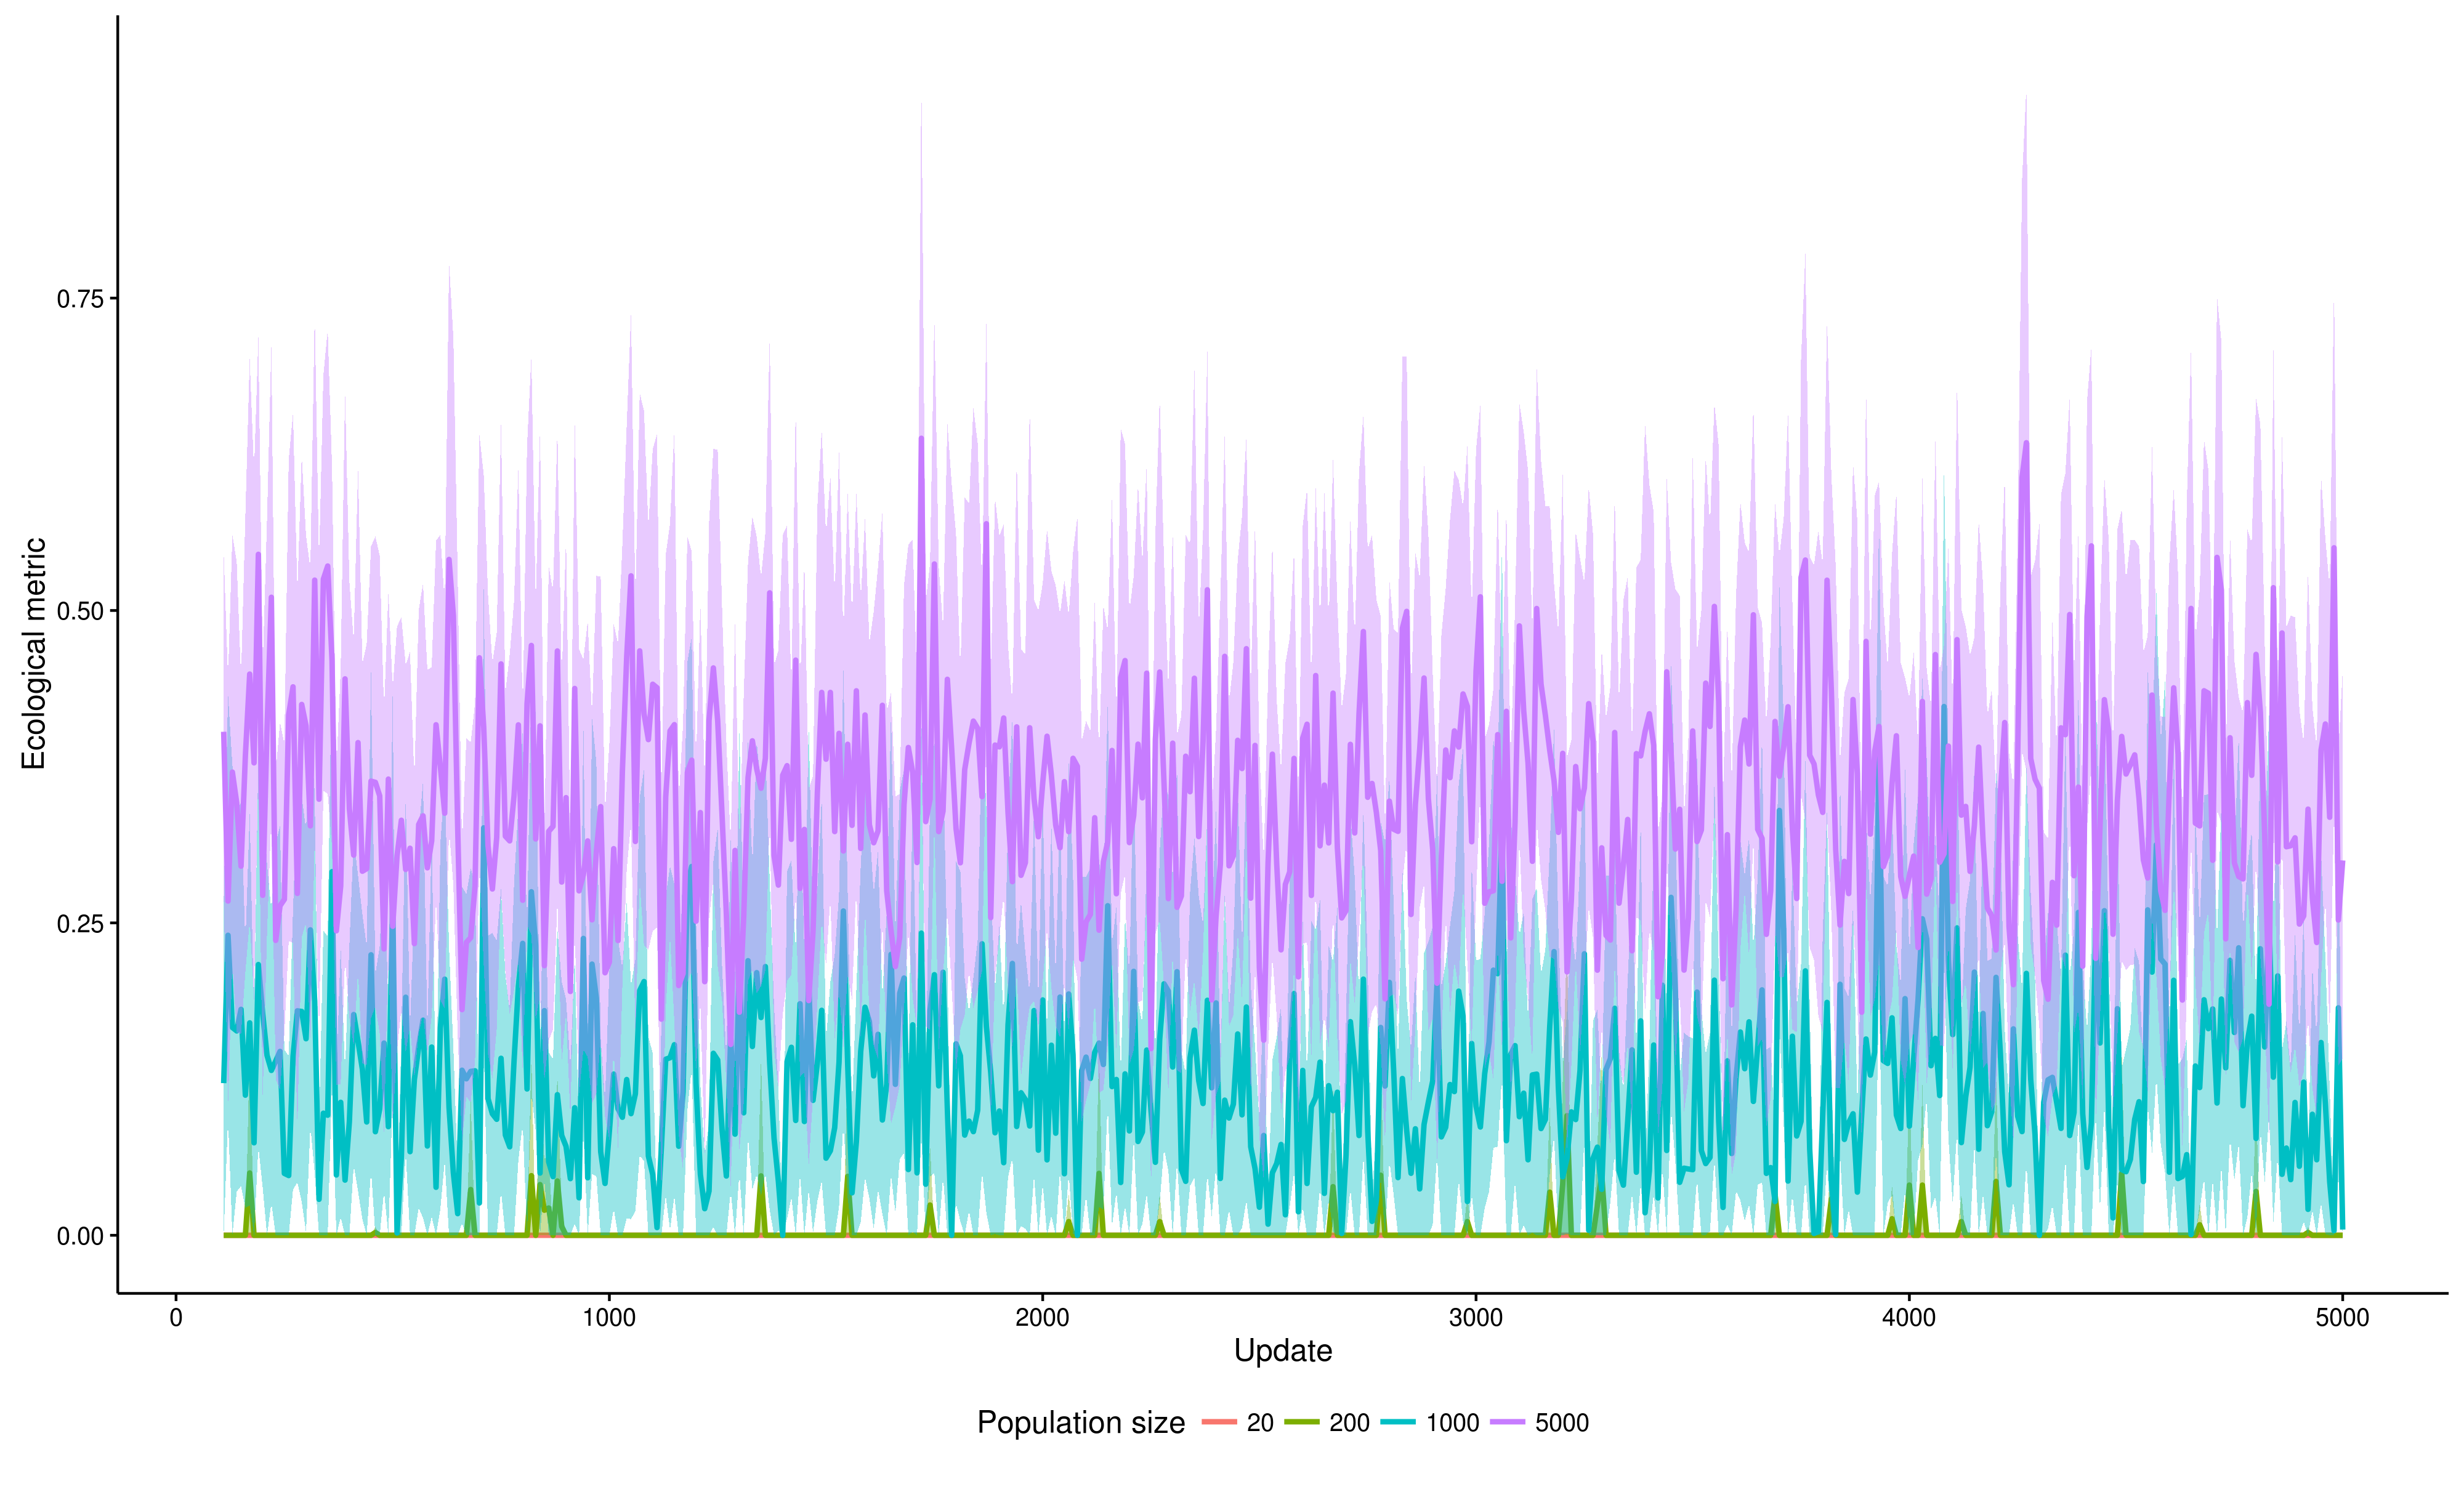
\includegraphics[width=3.5in]{figs/ecological_mean_ci_pop_size.png}
\caption{\textbf{Amount of ecology over time with varying population size.}}
\label{ecological_time}
\end{figure}
\begin{figure}
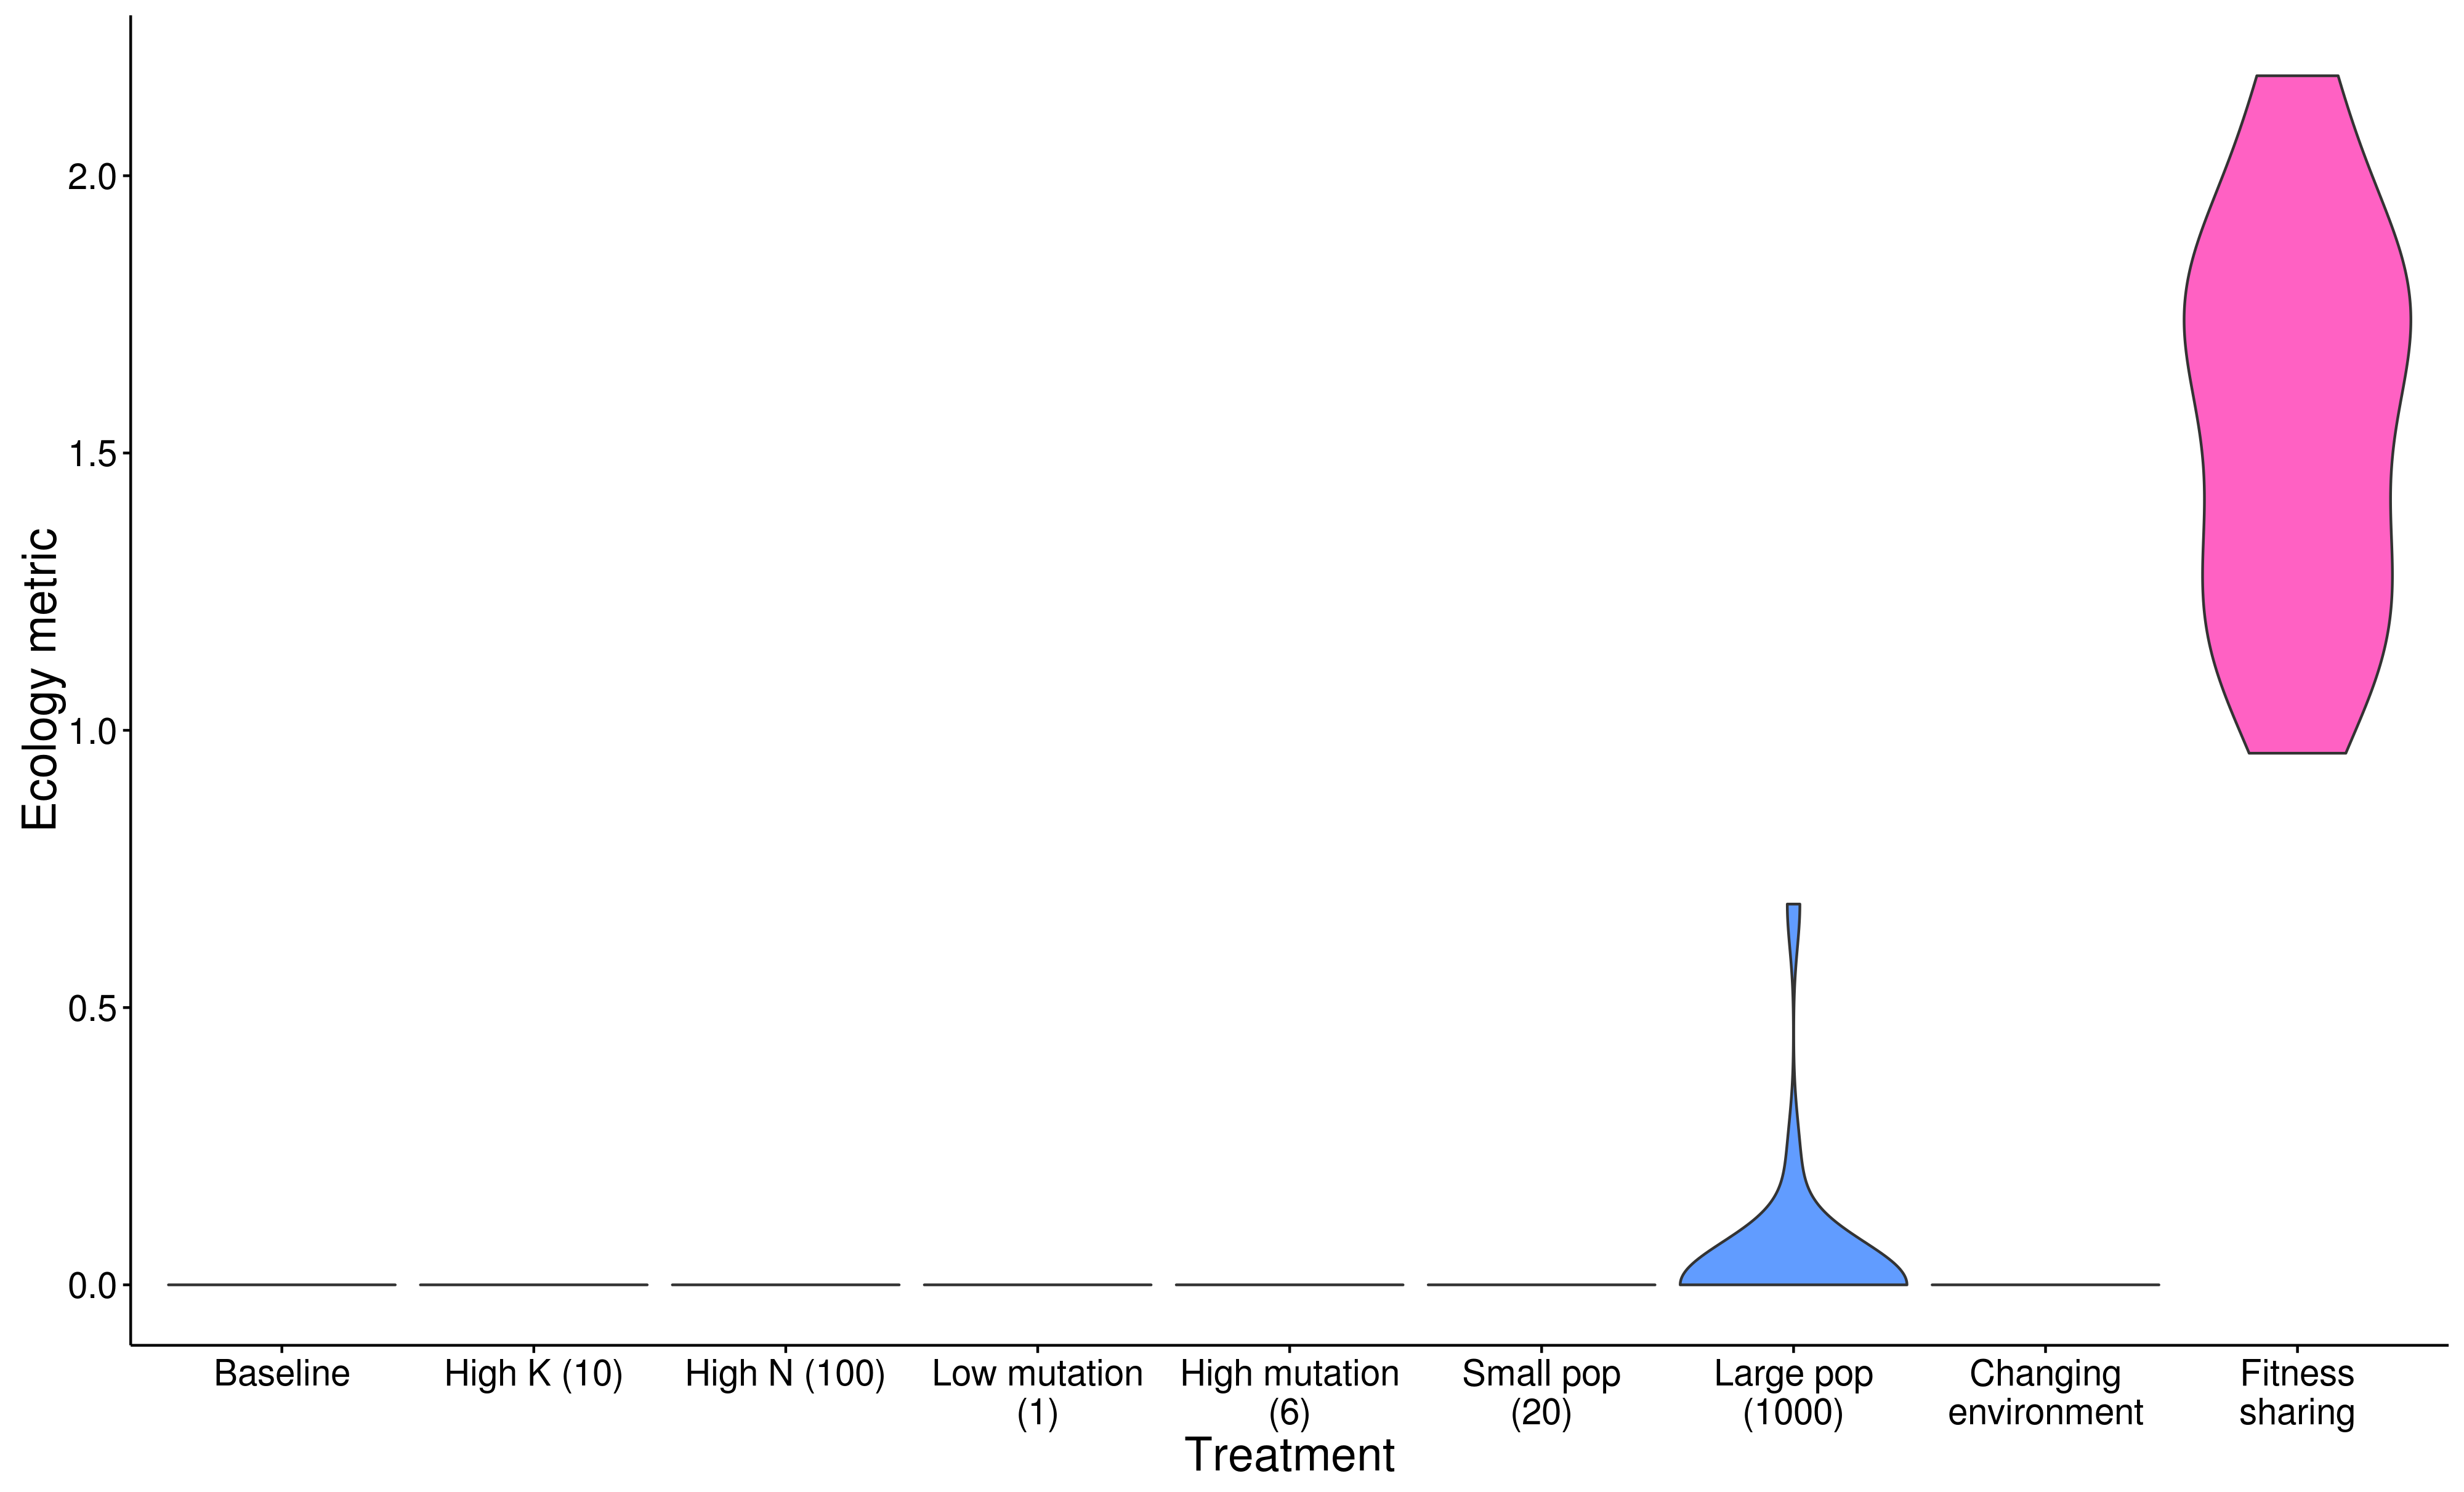
\includegraphics[width=3.5in]{figs/ecologyboxplots.png}
\caption{\textbf{Amount of ecology at final time point in varying environments.} }
\label{ecology}
\end{figure}



\section{Conclusions}
Though our simulation is fairly simple, it demonstrates that our metrics respond intuitively to the dynamics in a system. Thus, they should be able to detect systems that are theoretically capable of achieving open-ended evolution. First, it is clear that for new behaviors to evolve in a system, new genomes need to be evolving. Therefore, both the change and novelty metrics would need to be non-zero -- though they could be stable instead of increasing since both metrics measure a change. 
Second, continuously increasing complexity with a stable environment would imply increasing biotic interactions, potentially cooperative or complex competitive interactions. This implication is because if complexity is increasing in a population, at least one organism must be incorporating more information into its genome than any organism had before. This information can be about the environment up to a point. However, if the environment is not changing, complexity will not be able to increase unboundedly without biotic interactions between organisms. Therefore, continuously increasing complexity implies that interesting biotic interactions are evolving in a system, though they could be cooperative or competitive and likely include both.
Finally, a continuously increasing ecological metric in a stable environment implies an ecosystem is forming. This is because if the ecology metric is increasing, the informative diversity in the population is increasing. For diversity to be increasing, new niches must be emerging -- if there was only a single niche, the best genotype for that niche would fill it and take over the population. The only way for diversity to be maintained for a meaningful length of time is for new niches to be created. While new niches can emerge from abiotic factors, if the environment is not changing, those will eventually all fill. Therefore, the only way for an indefinite series of new niches to form (which is required for an unbounded increase of the ecological metric), there must be biotic interactions between organisms in the population. Those biotic interactions could fall into a number of categories such as predator and prey, mutualism, parasitism or commensalism, but as the number of them increase, a complex ecosystem emerges.

 More importantly, we can use these metrics to understand the impact of incremental changes to a system. In order to apply the scientific method to a monolithic problem like designing an open-ended evolutionary system, we need to be able to break that problem down into components that can be addressed in a systematic manner. Moreover, one of the primary goals in building such a system is to understand what components are necessary to do so. By looking at the effects that individual, controlled changes to a system have on this suite of metrics, we can more effectively work towards these goals.


Even biological systems like the LTEE

The metrics we propose here are applicable not only to digital systems, but are also relevant to experimental biological systems.  The Long-Term Evolution Experiment (LTEE) \citep{lenski_long-term_1991} is an exemplar of experimental evolution, consisting of 12 populations of the bacteria E. coli which have been evolving independently for more than 60,000 generations.  As detailed in \citep{taylor_open_inpress}, the LTEE exhibits many hallmarks of open-ended evolution, including the criteria we propose here.  Because fitness within the LTEE is best described by an unbounded power law function \citep{wiser_long-term_2013,lenski_sustained_2015}, the system meets the change metric; populations continue to change in non-trivial ways over time.  Studies of individual populations within the LTEE have shown numerous examples of generation of novelty, including exploration of new areas of the fitness landscape \citep{tenaillon_tempo_2016}, repeated selective sweeps \citep{maddamsetti_adaptation_2015}, new diversity arising after such sweeps \citep{blount_genomic_2012}, and epistasis between late mutations and those which arose earlier \citep{wielgoss_mutation_2013}, fulfilling the novelty metric.  Several populations within the LTEE demonstrate frequency-dependent fitness dynamics \citep{ribeck_modeling_2015,rozen_longterm_2000,le_gac_ecological_2012,maddamsetti_adaptation_2015}, which are necessarily cases of ecological interactions.  Included in these cases of frequency dependence is a special case \citep{blount_historical_2008,blount_genomic_2012,turner_replaying_2015} driven by crossfeeding and specialization on different resources \citep{turner_evolution_2015}.  Because all of the populations in the LTEE began as single cells, all ecological complexity in any populations must have arisen during the course of the experiment, and thus satisfies the  ecological metric.  The complexity metric is inherently harder to quantify in a biological system than in a computational one, but recent large scale genome sequencing from the LTEE \citep{tenaillon_tempo_2016} offers the promise of being able to measure complexity at the genome level over the course of the experiment.  The fact that our metrics work in a well-studied biological example of open-ended evolution lends greater credence to applying them computational studies as well.


\bibliographystyle{apalike}
\bibliography{bibliography}

\end{document}
